\documentclass[sigconf]{acmart}

% Remove this for camera-ready
\settopmatter{printacmref=false} % Removes citation information below abstract
\renewcommand\footnotetextcopyrightpermission[1]{} % removes footnote with conference information in first column
\settopmatter{printfolios=true}

\usepackage{times}
\usepackage[utf8]{inputenc}
\usepackage{url}
\usepackage{array,multirow}
\usepackage{xspace}
\usepackage{xcolor}
\usepackage{color, colortbl} 
\usepackage{balance}
\usepackage{paralist}
\usepackage{cleveref}
%\usepackage{amssymb}
\usepackage{graphicx}
\usepackage{pifont}
\usepackage{array}
\usepackage{booktabs}
\usepackage{tikz}
\usepackage{bm}
\usepackage{enumitem}
\setlength {\marginparwidth}{2cm}
\usepackage{todonotes}
\usepackage{arydshln}
\usepackage{makecell}
\usepackage{tabularx}
\usepackage{authblk}
\usepackage{caption}
\usepackage{soul,color}
%\usepackage{subcaption}
\usepackage{mwe}
\usepackage{ifthen}
\usepackage{algorithm}
\usepackage[noend]{algpseudocode}
\usepackage{epsfig}
\usepackage[tight,footnotesize]{subfigure}

\newcommand{\cmark}{\ding{51}}%
\newcommand{\xmark}{\ding{55}}%

%!TEX root = main.tex
%=========================================================

% use true/false to toggle all comments (both kinds)

\newboolean{showcomments}
\setboolean{showcomments}{false}

% ====== comments ======
\newcommand\important[1]{\todo[inline]{\textbf{Important:} #1}}
\newcommand\alberto[1]{\todo[color=yellow,inline]{\textbf{Alberto:} #1}}
\newcommand\etienne[1]{\todo[color=orange,inline]{\textbf{Etienne:} #1}}
\newcommand\pierre[1]{\todo[color=brown,inline]{\textbf{Pierre:} #1}}
\newcommand\felix[1]{\todo[color=blue!40,inline]{\textbf{Felix:} #1}}
\newcommand\michal[1]{\todo[color=green,inline]{\textbf{Michał:} #1}}
\newcommand\onur[1]{\todo[color=red,inline]{\textbf{Onur:} #1}}
\newcommand\sergi[1]{\todo[color=pink,inline]{\textbf{Sergi:} #1}}
\newcommand\ramin[1]{\todo[color=brown,inline]{\textbf{Ramin:} #1}}
\newcommand\mustafa[1]{\todo[color=brown,inline]{\textbf{Mustafa:} #1}}
% Uncomment the following command to make all comments disappear
\ifthenelse{\boolean{showcomments}} { }
{
\renewcommand\important[1]{}
\renewcommand\alberto[1]{}
\renewcommand\mustafa[1]{}
\renewcommand\michal[1]{}
\renewcommand\onur[1]{}
\renewcommand\sergi[1]{}
\renewcommand\etienne[1]{}
\renewcommand\pierre[1]{}
\renewcommand\ramin[1]{}
\renewcommand\felix[1]{}
}

% ====== inlined and toggable comments ======

\ifthenelse{\boolean{showcomments}}
{ \newcommand{\mynote}[3]{
    \protect\fbox{\bfseries\sffamily\scriptsize#1}
    {\small\textsf{\emph{\color{#3}{#2}}}}}}
{ \newcommand{\mynote}[3]{}}

\newcommand{\er}[1]{\mynote{Etienne}{#1}{blue}}
\newcommand{\mk}[1]{\mynote{Michał}{#1}{brown}}
\newcommand{\sr}[1]{\mynote{Sergi}{#1}{red}}

% \newcommand{\xxx}[1]{\mynote{YourName}{#1}{black!20!red!80!}}
% \newcommand{\xxx}[1]{\mynote{YourName}{#1}{green}}
\newcommand{\as}[1]{\mynote{Alberto}{#1}{orange}}
\newcommand{\dk}[1]{\mynote{Daniel}{#1}{green}}
\newcommand{\rs}[1]{\mynote{Ramin}{#1}{violet}}
\newcommand{\oa}[1]{\mynote{Onur}{#1}{red}}

% ====== systems ======
% \newcommand\sysname{TOPDISC\xspace}
\newcommand\sysname{DISCv5\xspace}
\newcommand\discv{DISCv4\xspace}
\newcommand\altname{DHT\xspace}
\newcommand\altnameticket{DHTTicket\xspace}
\newcommand\altsysname{PMETIS\xspace}
\newcommand\sysnamePriv{Pineapple\xspace}
\newcommand\sysnameAnon{\coconut}
\newcommand\libcoin{LibraCoin\xspace}
\newcommand\libcoins{LibraCoins\xspace}
\newcommand\privcoin{PrivCoin\xspace}
\newcommand\privcoins{PrivCoins\xspace}

\newcommand\sysnamereplay{\texttt{byzcuit}\xspace}
\newcommand\sysnamebaseline{\texttt{byzcuit-baseline}\xspace}
\newcommand\simplesysname{Simple-\sysname}

\newcommand\libra{Libra\xspace}
\newcommand\fourier{Fourier\xspace}
\newcommand\chainspace{Chainspace\xspace}
\newcommand\ethereum{Ethereum\xspace}
\newcommand\hyperledger{Hyperledger\xspace}
\newcommand\omniledger{Omniledger\xspace}
\newcommand\rapidchain{RapidChain\xspace}
\newcommand\elgamal{El-Gamal\xspace}
\newcommand\coconut{Coconut\xspace}
\newcommand\macggm{$\bm{\mathrm{MAC_{GGM}}}$\xspace}
\newcommand\sbac{S-BAC\xspace}
\newcommand\bft{BFT\xspace}
\newcommand\atomix{Atomix\xspace}
\newcommand\cscoin{CSCoin\xspace}
\newcommand\rscoin{RSCoin\xspace}
\newcommand\lsbac{\sysname}
\newcommand\fsbac{F-SBAC\xspace}
\newcommand\bftsmart{\textsc{bft-SMaRt}\xspace}

\makeatletter
\def\BState{\State\hskip-\ALG@thistlm}
\makeatother

% ====== custom notations ======
%\newcommand\algorithm[1]{\textsf{#1}}
\newcommand\hashtopoint{H^*\xspace}
\newcommand\stringtopoint{H'\xspace}
\newcommand\function[1]{\ding{118}\xspace \textsf{#1}:\xspace}
\newcommand\shard[1]{\emph{shard}\xspace#1\xspace}
\newcommand\Shard[1]{\emph{Shard}\xspace#1\xspace}
\newcommand\preacceptt{\textsf{pre-accept}($T$)\xspace}
\newcommand\preabortt{\textsf{pre-abort}($T$)\xspace}
\newcommand\preaccepttt{\textsf{pre-accept}($T'$)\xspace}
\newcommand\preaborttt{\textsf{pre-abort}($T'$)\xspace}
\newcommand\preacceptttt{\textsf{pre-accept}($T''$)\xspace}
\newcommand\preacceptts{\textsf{pre-accept}($T,s_T$)\xspace}
\newcommand\preabortts{\textsf{pre-abort}($T,s_T$)\xspace}
\newcommand\preabortttt{\textsf{pre-abort}($T''$)\xspace}
\newcommand\acceptt{\textsf{accept}($T$)\xspace}
\newcommand\abortt{\textsf{abort}($T$)\xspace}
\newcommand\accepttt{\textsf{accept}($T'$)\xspace}
\newcommand\aborttt{\textsf{abort}($T'$)\xspace}
\newcommand\acceptttt{\textsf{accept}($T''$)\xspace}
\newcommand\abortttt{\textsf{abort}($T''$)\xspace}
\newcommand\acceptts{\textsf{accept}($T,s_T$)\xspace}
\newcommand\abortts{\textsf{abort}($T,s_T$)\xspace}
\newcommand\myrow[1]{row\xspace\textsf{#1}\xspace}
\newcommand\mycolumn[1]{column\xspace\textsf{#1}\xspace}
\newcommand\shardled{shard-led\xspace}
\newcommand\Shardled{Shard-led\xspace}
\newcommand\clientled{client-led\xspace}
\newcommand\Clientled{Client-led\xspace}
\newcommand\activeObj{`active'\xspace}
\newcommand\inactiveObj{`inactive'\xspace}
\newcommand\locked{`locked'\xspace}
\newcommand\wa{{WA}\xspace}
\newcommand\wb{{WB}\xspace}
\newcommand\ka{{KA}\xspace}
\newcommand\kb{{KB}\xspace}

% ====== concepts/terminology =======

\newcommand\attacker{attacker\xspace}
\newcommand\adversary{attacker\xspace}
\newcommand\prerecorded{prerecorded\xspace}
\newcommand\prerecords{prerecords\xspace}
\newcommand\prerecord{prerecord\xspace}

%  ===== formatting ======
% Abbreviations etc.
\newcommand{\cf}{cf.\@\xspace}
\newcommand{\vs}{vs.\@\xspace}
\newcommand{\etc}{etc.\@\xspace}
\newcommand{\ala}{ala\@\xspace}
\newcommand{\wrt}{w.r.t.\@\xspace}
\newcommand{\etal}{\textit{et al.}\@\xspace}
\newcommand{\eg}{\textit{e.g.}\@\xspace}
\newcommand{\Eg}{\textit{E.g.}\@\xspace}
\newcommand{\ie}{\textit{i.e.}\@\xspace}
\newcommand{\Ie}{\textit{I.e.}\@\xspace}
\newcommand{\via}{\textit{via}\@\xspace}
\newcommand{\defacto}{\textit{de facto}\@\xspace}

\newcommand\mypara[1]{\vspace{0.05in} \noindent \textbf{#1.}}
\newcommand\para[1]{\vspace{0.05in} \noindent \textbf{#1.}}


\newcommand\definition[2]{\ding{118}\xspace \textsf{#1}\xspace$\bm{\rightarrow}$\xspace(#2):\xspace}



% For inlined section titles.
\newcommand\inlinesection[1]{{\bf #1.}}

\def\first{({\it i})\xspace}
\def\second{({\it ii})\xspace}
\def\third{({\it iii})\xspace}
\def\fourth{({\it iv})\xspace}
\def\fifth{({\it v})\xspace}
\def\sixth{({\it vi})\xspace}

\newcommand{\one}{({\em i})\xspace}
\newcommand{\two}{({\em ii})\xspace}
\newcommand{\three}{({\em iii})\xspace}
\newcommand{\four}{({\em iv})\xspace}
\newcommand{\five}{({\em v})\xspace}

% Colours
\definecolor{verylightgray}{gray}{0.8}

% Table
\newcolumntype{L}{l<{\hspace{1cm}}}
\newcolumntype{C}{c<{\hspace{1cm}}}
\newcolumntype{D}{c<{\hspace{0.3cm}}}

% Markers
\newcommand\vgap{\vskip 2ex}
\newcommand\marker{\vgap\ding{118}\xspace}

\def\na{--}
\def\unsure{?}
\def\missing{$!$}
\newcommand{\yes}{\ding{51}}
\newcommand{\no}{\ding{55}}
\DeclareRobustCommand\pie[1]{
\tikz[every node/.style={inner sep=0,outer sep=0, scale=1.5}]{
\node[minimum size=1.5ex] at (0,-1.5ex) {}; 
 \draw[fill=white] (0,-1.5ex) circle (0.75ex); \draw[fill=black] (0.75ex,-1.5ex) arc (0:#1:0.75ex); 
}
}
\def\L{\pie{0}} % Low
\def\M{\pie{-180}} % Medium
\def\H{\pie{360}} % High


\begin{document}

\title{Topic-based service discovery for the Ethereum P2P network}
\author{}


\begin{abstract}
Abstract
\end{abstract}

\maketitle
%!TEX root = ../main.tex
%=========================================================

\section{Introduction}
\para{Motivation} Ethereum~\cite{buterin2013ethereum}  is one of the largest permissionless,  open-source  blockchains supporting Turing-complete scripting via smart contracts. Ethereum runs a Peer-to-Peer (P2P) network based on Kademlia Distributed Hash Table (DHT) ~\cite{maymounkov2002kademlia} to exchange pending transactions and mined blocks. 

%Following its decentralized design, Ethereum relies on a Peer-to-Peer (P2P) communication network, where individual nodes, running an Ethereum client software (\eg Go Ethereum~\cite{go-ethereum}), send and receive messages containing transactions and blocks to achieve distributed consensus, without relying on any central node or a trusted third party. The core system and the associated protocols used by the peers to participate in the Ethereum P2P network is included as part of a suite called DEVp2p. The suite includes individual sub-systems and protocols for services such as node discovery or establishing secure or point-to-point communication between peers. 

Apart from supporting blockchain data exchange, the Ethereum P2P network is also used by other applications. This includes multiple Ethereum testnets (Ropsten, Rinkeby),  alternative cryptocurrencies(Pirl, Musicoin) and other decentralized platforms such as iExec or Swarm.
In 2018, the Ethereum P2P network nodes operated a total of 4,076 different applications\cite{kim2018measuring}. Most of those applications require a dedicated P2P network to disseminate application-specific messages (\eg event notifications) to the interested peers but rely on the larger, Ethereum P2P network for bootstrapping.

Using an existing, well-established P2P network to bootstrap smaller, application specific networks has multiple advantages. Firstly, it encourages re-using reliable code to perform common tasks such as securing connections or finding peers. Secondly, P2P network security increases with the number of its honest participants. Being part of a larger swarm makes smaller applications more resistant to various attacks\hl{some refs from attack of smaller blockchains}. Finally, application developers can focus uniquely on implementing application-specific services boosting the growth of the entire, decentralised ecosystem. 

To realise this vision, nodes must \textit{(i)} join a larger, host P2P network, \textit{(ii)} discover their application-specific peers, \textit{(iii)} form an application-specific network. However, peer discovery in a fully decentralised setup is a challenging task. Unlike existing discovery protocols that work in a local setting (MDNS/Bonjour\hl{[?]}) or rely on trusted operators \hl{[?]}, decentralised node discovery must work at a global scale and in a fully decentralised setting. Due to the high heterogeneity of applications and (potentially constraint) peers, such a protocol must be efficient and introduce low communication and computational overhead. Finally, an open system, must protect against malicious actors trying to disturb network services, exhaust resources of honest peers or hijack application-specific networks. 

\para{State of the art} In the current Ethereum service discovery system, \ie discovery version 4 (Discv4), nodes perform a \textit{brute-force} discovery process. A node willing to discover application-specific peers randomly traverses the DHT and initiates connections with all the encountered nodes. A permanent connection is established only if a peer supports the same application and terminated otherwise. Such an approach provides strong security guarantees but results in a large communication overhead and long discovery times, particularly for unpopular applications with a small number of peers. While multiple, alternative discovery systems have been proposed \hl{[?]}, they rely on unrealistic assumptions \hl{[?]}, introduce high overhead or fail to operate in a presence of an adversary \hl{[?]}. 

\para{Discv5} In this work, we propose a new \textbf{service discovery sub-system} which enables secure,  efficient and robust  discovery of application-specific peers in the Ethereum network,  that will be part of the new DEVp2p  discovery system version 5 (\textit{\sysname}).
Different from Discv4, \sysname allows nodes (\ie advertisers) to associate themselves with a set of \emph{topics} (\eg application IDs), and advertise the association (\ie an ad) to the network. The information is collectively stored by network participants (\ie registrars) without relying on a single trusted party at any point. Any node can then query the network for a topic to obtain a list of application-specific peers and directly connect to them without disturbing other members of the network. 

We build \sysname on top of the existing Ethereum DHT to avoid major changes to the system and take advantage of the already existing routing infrastructure. The protocol propagates application-specific advertisements to multiple nodes chosen in an unpredictable way to protect against targeted attacks. Our design encourages diversity of advertisements stored at each registrar making the system resistant to network dynamics. At the same time, \sysname provides efficient peer discovery operations terminating within a bounded number of steps for all the topics regardless of their popularity. The protocol implements a robust admission mechanism to limit the resource usage on all the nodes, ensure fairness across topics, and prevent a vast range of malicious behaviours even in the presence of a powerful attacker.

\para{Contributions} We make the following contributions:
\begin{itemize}
    \item In \Cref{sec:placement}, we design a DHT-based data placement system that distributes service advertisement in the network. The protocol combines pseudo-random data placement for security with deterministic operations for efficiency. We present a lookup operation that finds a subset of advertisement placed in the system within a bounded amount of time. The procedure ensure the diversity of data sources and is resistant against manipulation by malicious registrars. 
    \item In \Cref{sec:registration} we design a lightweight admission protocol allowing advertisers to place ads after waiting for a specified amount of time. \sysname guarantees that advertisers cannot place more advertisement by deviating from the protocol and does not create any intermediary state at nodes holding the advertisements. 
    \item In \Cref{sec:waitingTime}, we design a function that calculates a waiting time after which advertisement can be placed on nodes holding advertisements. The function limits the amount of resources used by each node, promotes ads diversity stored within nodes, and protects against a vast range of malicious behaviours. 
\end{itemize}

In \Cref{sec:eval}, we evaluate \sysname under different system parameters and against state-of-the-art decentralised discovery systems. Our system achieves better load-balancing and requires more resource consumption by the attackers to successfully launch attacks such as eclipsing attacks. We also provide performance evaluation results from both simulations and from real system deployment. \sysname is scheduled for implementation in the next version of the Ethereum P2P network. 

%\michal{From the paragraph below we should form a requirements parts}
% An open and decentralized discovery system introduces new security challenges that need to be addressed. Malicious nodes may decide to deviate from the protocol in order to increase their own visibility or disrupt system operations. A particularly important security challenge is the \textit{Sybil attack} which can amplify the attacking power of malicious nodes, typically with very little resource consumption. The Sybils can launch various attacks including Denial-of-Service (DoS) by ignoring ad lookups, spam ads with bogus topic advertisement, and launch more sophisticated attacks to isolate nodes from their peers in their target sub-networks (\ie eclipse attack). 
%\michal{The above needs completion}
%\ramin{Is the above information about attacks needed in the introduction?}
%\michal{Probably not. We must just say there are problems with security}




%%!TEX root = ../main.tex
%=========================================================

\section{Introduction}

Ethereum~\cite{} is a decentralized, open-source blockchain for distributed computing, allowing users to develop various decentralized applications (DApps).  Ethereum  was the first major blockchain to support Turing-complete scripting via smart contracts, Ethereum also operates as a cryptocurrency by supporting the transfer of tokens called ether between Ethereum accounts.
In addition to its use as a fiat currency,  ether is also used to incentivize Ethereum nodes to perform distributed computation. 
Ether can also be converted to gas, which is used as a fee for executing transactions and smart contracts, and effectively mitigates spam. 

Ethereum is the most actively used blockchain~\cite{bloomberg} nowadays.
Following its decentralized design and structure, Ethereum relies on a communication infrastructure provided by a peer-to-peer (P2P) network, where individual and independent nodes, running an Ethereum client software (e.g., Go Ethereum~\cite{go-ethereum}), send and receive messages  containing transactions and blocks to achieve distributed consensus,  without relying on any central node or a trusted third party.

The set of network protocols which form the Ethereum peer-to-peer network are called DEVp2p.  DEVp2p isn't specific to a particular blockchain, but should serve the needs of any networked application associated with the Ethereum umbrella.
Other protocols can also run on top of DEVp2p,  such as 
The Whisper protocol~\cite{} (for decentralized
applications) and the Swarm protocol~\cite{} (for decentralized file
storage).
DEVp2p provides peers connection management and also node discovery services.
%Between the DEVp2p network protocols and the app protocol (i.e., Ethereum, Whisper, Swarm, etc), RLPx~\cite{} provides a secure transport layer. 
%\michal{The above seems too detailed IMO. We can introduce DEV2p, RLPx etc. in the background. I'd only say that Ethereum DHT can be used by other services (not necessarily blockchain related) and give some examples.}

DEVp2p is the responsible of managing the connections to other peers which form the overlay P2P network.
%For instance,  Go-ethereum client by default establish a total of 50  connections to other Ethereum nodes.  Of these 50 slots,  two thirds are reserved for inbound connections (initiated by other peers),  while the remaining third are allocated for outbound connections. 
%No further restrictions apply to inbound connections; if an inbound slot is available
%Go-ethereum client simply accepts any connecting peer that supports the
%Ethereum protocol and operates on the same network (main,
%testing, etc.). 
%The outbound slots are therefore selected by the nodes, which need to be done carefully to avoid any attacker could mount an eclipse attack.
%In an eclipse attack, an
%adversary monopolizes the connections of a victim, effectively
%filtering the victim’s view of the blockchain.  Eclipse attacks
%enable a variety of follow-up attacks such as double spending
%and stubborn mining~\cite{}.
%\michal{ditto}
In order to find and select participants of the P2P network to initiate connections to,  a node discovery protocol is required by DEVp2p.
Systems such as MDNS/Bonjour allow finding hosts,  but only in  a local-area network.  
However, DEVp2p discovery protocol requires to work on the Internet and to be useful for applications with a large number of participants spread across the Internet.
There are systems that uses a rendezvous server for network discovery over the Internet,  such as desktop applications or cloud services. 
But using rendezvous servers requires trust in the operator and these systems are prone to censorship. 
For a decentralized network,  such as the Ethereum network,  it is not desirable to rely on a single operator.  
Instead,  it is better to place a small amount of trust in every participant, becoming more resistant to censorship as the size of the network increases and participants of multiple networks can share the discovery network to further increase its resilience.
%The process of joining the network is the Achilles heel of the node discovery protocol: while any other node may be used as an entry point,  such a node must first be located through some other mechanism.  
%Approaches such as listing of initial entry points in DNS or discovery of participants in the local network can be used,  but only as a reasonable secure entry into the network.

Current version of DEVp2p distributed node discovery protocol is discovery version 5 (Discv5).
Node discovery protocol can be used by any node on the network  at no cost other than running the network protocol and storing a limited number of other nodes' records. 
Any node can be used as an entry point into the network.
Discv5 system's design is loosely inspired by the Kademlia DHT~\cite{}.
%In Kademlia DHT,  information about known overlay nodes is stored in
%a distributed table separated into so-called k-buckets (or simply buckets),  where each bucket stores nodes identifiers within the same distance to the local node id.
%But unlike most DHTs no arbitrary keys and values are stored. 
%Instead, the DHT stores and relays 'node records', which are signed documents providing information about nodes in the network. 
Discv5 acts as a database of all live nodes in the network %and performs three basic functions:
and,  by walking the DHT,  all nodes of the network can be discovered and enumerated.

%\begin{itemize}
% \item Sampling the set of all live participants: by walking the DHT,  the network can be enumerated.
% \item Searching for participants providing a certain service: Discv5 includes a scalable facility for registering 'topic advertisements'. These advertisements can be queried and nodes advertising a topic found.
% \item Authoritative resolution of node records: if a node's ID is known, the most recent version of its record can be retrieved.
%\end{itemize}

The concept of topic is a new concept in Discv5 (compared with previous node discovery protocol -Discv4-),  
Discv5 will allow nodes to associate themselves with a set of tags, i.e., topics, and enable searching of peers that advertise themselves as associated with particular topics.  
Topics can be used to identify different  capabilities, for instance specific application capabilities,  services or certain functionalities of a node. 
\hl{Topics example missing}
Topic based peer finding is a promising feature because it allows a potential bandwidth reduction and much faster discovery of nodes
by  discovering nodes based on the topic required.
This means that instead of connecting to every node discovered to see if it offers a specific service,  a node can simply lookup for nodes that are only providing the service and then ask them if they really are still offering the service.
This will avoid a waste of time and resources by leaving apart those nodes that do not declare the service in its capabilities,  avoiding handshakes node by node to discover these details and relying only on the node discovery protocol. 

However,  Discv5 still lacks of mechanisms to register and discover nodes for specific topics.
Providing new mechanisms for registering and discovering for specific topics in Discv5 is challenging because of the decentralized structure of the network and its vulnerability to Sybil attacks~\cite{} (any node joining the network can be a malicious node) adds complexity to any proposed solution that has to work for any kind of service despite its popularity.

%\michal{I'd write the intro on a higher level. E.g., 1) Ethereum is the largest network/blockchain 2) It is fully decentralized and decentralization is great 3) Ethereum allows hosting multiple services other than Ethereum blockchain) and uses Ethereum DHT as a communication/management platform 4) A crucial part of that is to enable nodes working with the same application to find each other 5) this is challenging because of decentralization/security/malicious can join etc. 6) State of the Art doesn't work (briefly - we have better analysis in related work) 7) We propose our brand new shiny protocol that is efficiency and secure 8) Our contributions + structure}


%It is envisioned that the Discv5 system will be used across many different services at large scale, mainly to form subnetworks consisting of the service peers.  The basic objectives of Node Discovery v5 is to provide a facility for nodes to i) register 'topic advertisements', i.e., “ads”, at other peers in the Ethereum network and ii) find other nodes that advertised a particular topic by querying selected peers in the Ethereum network.

The goal of this paper is to propose and evaluate a new mechanism for the Discv5 protocol for registering and discovery nodes in the network for a certain topic,  integrating it in the existing DEVp2p node discovery protocol based on Kademlia DHT.  
The new mechanism is capable of registering and discovering for services in the Ethereum P2P network efficiently for any service regardless of the popularity of the service, using a bounded number of hops and resistant to Sybil attacks.
\hl{Any missing nice feature of the proposal}.

The mechanisms proposed are the following:

\begin{itemize}
 \item New registering mechanism that register nodes only for the topics that matches nodes capabilities.
 \item New table structure on top of the existing Kademlia DHT to store node information based on topics advertised.
 \item New lookup mechanism that discover nodes based on the topics advertised in the P2P network.
\end{itemize}
    
The structure of the paper is the following....\hl{TBC}


\section{Background}\label{sec:background}
\michal{Need a good introduction on Kademlia here. Distances/buckets etc. It's required to explain the ticket table, routing etc.}

%!TEX root = ../main.tex
%=========================================================

\section{System and threat models}
\label{sec:model}

\begin{table}
    \caption{Notation}
    \label{tab:notation}
\begin{center}
    \begin{tabular}{ | l | p{8cm} |}
      \hline
        $N$ & network size \hl{Consider changing to all nodes so that $n \in N$} \\ \hline
        $k$ & number of peers holding a key in the DHT (from the background section) \hl{not sure we need it - it's only in the background and we can explain everything by finding just 1 closest peer to the key} \\ \hline
        $X$ & a node (from the background section) \\ \hline
        $n$ & \hl{a node (from the 4.1)} \\ \hline
        $n$ & total size of the ad cache (Sec. 5.2) \hl{a clash with node} \\ \hline
        $p$ & peer (section 4.1) \\ \hline
        $T$ & Table (section 4.1) \\ \hline
        $b_i$& $i$-th bucket (section 4.1) \hl{TODO: add key} \\ \hline
        $\alpha$ & number of concurrent routing operations \\ \hline
        $K_{\textit{register}}$ & number of ads placed per bucket\\ \hline
        $K_{\textit{lookup}}$ & \hl{It's weirdly defined in Sec. 4.4}: search process progresses using maximum $K_{\textit{lookup}}$  parallel requests, and issuing requests towards up to $K_{\textit{lookup}}$  peers per bucket.\\ \hline
        $a$ & ad lifetime  (Sec. 4.3)\\ \hline
        $N_{\textit{lookup}}$ & number of peers to find (Sec. 4.4) - \hl{could be introduced before specifying what the system does} \\ \hline
        $N_{\textit{return}}$ & max number of topic-specific peers returned from a single registrar \\ \hline
        $t_{\textit{init}}$ & ticket: the local time at the registrar when the ad was received for the first time \\ \hline
        $t_{\textit{waiting}}$ & ticket the local time at the registrar when the ad was received for the first time \\ \hline
        $\delta t_{\textit{window}}$ & registration window \hl{we probably don't need both $\delta$ and "window"} \\ \hline
        $t_{\textit{cumulative}}$ & ticket:cumulative waiting time \\ \hline
      \hline
    \end{tabular}
  \end{center}
\end{table}
\mk{TODO: add notation for number of malicious nodes, number of malicious IPs etc.,}
\mk{change bucket definition to add the target key (can be useful to define advertise tables etc. if we introduce them in the background \eg $b_i(key)$). We also often indicate the farthest buckets - we could simply use $b_0$}
\mk{Put macros for the notation}
\mk{We need a notation for an ad - at the end of Sec. 5.2 we just use "Ad".}


In this section, we present our network and threat models as well as the target properties of \sysname. 

\subsection{System model}

We assume a network of $N$ nodes.\footnote{$N$ is unknown to the participants but is used in our analysis.}
At startup time, each node generates a public/secret key pair, which it uses to secure point-to-point communication with its peers.
Nodes are identified by their \emph{node ID}, which is simply the hash of their public key.
Multiple nodes may share the same IP address (due to NAT or being hosted by the same physical machine)~\cite{marcus2018low}.
However, two nodes cannot share the same ID.

% \er{revise: It is not clear \sysname is an extension of discv5 from the online documentation, but rather its central mechanism. What are the other protocols as part of discv5  is also unclear.}
% \sysname is built on the existing Ethereum DHT. Specifically, we designed and implemented our system as an extension of Ethereum's \emph{Node Discovery Protocol v5 (discv5)}. However, the operation of service discovery is not Ethereum-specific and could also be implemented using a different DHT. \er{I would not necessarily make this claim here, since several operations are. Kademlia-specific in reality. Maybe save for the conclusion?}

As for \discv, \sysname leverages the existing Ethereum DHT, but does not rely on its key lookup operations.
\sysname indexes different applications in the Ethereum eco-system as \emph{topics}.
A topic is an identifier for an application, or \emph{service}, provided by a node.
Topics are arbitrary strings that hash to a specific key. % in the DHT key space.

All DHT nodes fulfill the following roles:
\begin{itemize}
    \item A \textbf{registrar} accepts advertisements (\emph{ads}) and responds to topic queries. 
    When asked for a specific topic, a registrar responds with nodes that registered ads for this topic.
    % All DHT nodes act as registrars. 
    A registrar may accept and store ads for any topic.
    \item An \textbf{advertiser} registers for a specific service topic and wants to be discovered by its peers.
    Advertisers make themselves discoverable by placing ads for that topic.
    Nodes are advertisers for every service they participate in.
    \item A \textbf{searcher} attempts to discover nodes registered under a specific topic, using service lookup operations.
\end{itemize}

A node providing a certain service topic is said to \emph{register} itself when it submits an ad to a registrar. % to make itself discoverable under that topic.
Depending on the needs of the application, a node can advertise multiple topics or no topics at all. 
We assume that the popularity of topics in the system is highly heterogeneous, i.e., it can follow a power law distribution~\cite{kim2018measuring}.
Anyone can participate in registering and searching for (one or more) topics and use the same ID and IP for all its topics. 

\subsection{Threat Model}
\label{sec:threat}

\sysname is designed to operate in an open, adversarial environment.
We assume the presence of malicious actors in the network that may arbitrarily deviate from the protocol and coordinate their actions.
Malicious actors can spawn multiple virtual nodes within one physical machine, and operate multiple physical machines.
As a result, they can control a number of Sybil node IDs.

% \er{should we mention collusions here? It is mentioned only at the end of the section (although we do not seem to consider it so much in the experiments)}\mk{In the experiments we assume that all the Sybils ae controlled by a single entity. I've expanded the phrase above. I hope it's fine now.}
% % These actors do not strictly follow the protocol when communicating with others and attempt to influence the discovery results of honest nodes by steering them toward the attacker-controlled nodes.

The security of the service discovery mechanism is fundamentally dependent on the security guarantees provided by the underlying DHT implementation, and in particular on its ability to avoid eclipse attacks against a specific node.
Indeed, even if \sysname does not rely on DHT lookup operations, information in the DHT routing table is used to initialize and maintain the data structures used by the service discovery layer.
We assume, therefore, that no honest node is fully eclipsed by the malicious ones, \ie, each honest DHT node has \emph{at least} one honest peer.
As previously mentioned, Ethereum already implements multiple mechanisms preventing eclipse attacks at the DHT level~\cite{marcus2018low, henningsen2019eclipsing}.  

Maintaining nodes in the DHT requires infrastructure resources (public IP addresses) and we assume that the resources under the control of an attacker are limited.
Specifically, we assume that it is easier for an attacker to generate similar IP addresses (\ie within a single subnet) than it is to control many diverse IP addresses (with different prefixes).
We use the number of IP addresses and IDs under the control of an attacker as parameters for our evaluation in \Cref{sec:eval}.

\mk{We can probably remove those and mention those problems when introducing our system.}
Through a literature review~\cite{chen2020survey, henningsen2019eclipsing} we collected a list of malicious behaviors that an attacker can use to disrupt a DHT-based service discovery protocol:
\begin{itemize}
    \item \textbf{Malicious DHT Peer}: DHT routing relies on asking peers for other nodes, closer to a specific target. When responding to such requests, an attacker only returns other malicious nodes, in order to hijack the process of DHT traversal by honest nodes. \er{this seems contradictory with the fact that we wrote two paragraphs ago that we assumed the DHT to be secured against Sybils. Should we change DHT routing to something more generic, like an exploration process?} \er{also, this may appear contradictory to the fact we do not use the DHT routing (lookup) directly but implement our own}
    \item \textbf{Malicious Registrar}: When queried for a specific topic, an attacker returns a maximum amount of malicious nodes.\footnote{Alternatively, a malicious registrar could simply refuse to respond. However, such behavior is less effective than returning malicious peers.}
    \item \textbf{Spamming Advertisers}: An attacker bombards honest registrars with malicious ads. The attack can target single or multiple topics. The attack may cause an honest registrar to refuse honest ads due to lack of resources (\eg, storage and CPU power). This registrar will, furthermore, later return maliciously-inserted ads of the spammer when queried by honest searchers. 
    \item \textbf{Generic Spammers}: An attacker bombards an honest registrar with topic queries or random traffic hoping to exhaust bandwidth or CPU power.
\end{itemize}

Adversaries can strategically target specific nodes or regions in the DHT key space (\ie by generating Sybil Node IDs within the desired region) when implementing these attacks.
We assume the presence of attackers that can combine some or all of the behaviors above, and coordinate their actions to maximize their effect. 

\subsection{Target Properties}

Under the considered threat model, \sysname achieves the following properties.

\para{Efficiency} 
\sysname ensures that the number of nodes contacted and the number of messages exchanged increase logarithmically with the number of system participants, for both lookup and register operations. 
Sending and processing service discovery requests requires only simple operations involving a constant amount of resources.
The storage usage for the registrars is limited by a configurable but fixed cap that does not depend on the amount of incoming traffic. 

\para{Fairness}
\sysname ensures a balanced load distribution across systems participants and regions of the key space (\ie, it avoids \emph{hotspots}).
The system provides efficient lookup and registration operations for all participants regardless of the topic they look up or register for.
Each advertiser has a similar probability of being discovered by its peers. 
% \er{we should ideally be a bit more formal here and give bounds (in big O?) of the unbalance between these nodes.}\mk{What fairness metric would you suggest here?} \er{this would be ratio between the likelihood of being discovered for a popular and a less-popular advertiser}

\para{Security}
\sysname focuses specifically on preventing \emph{Denial of Service} (nodes are unable/slow to discover their application-specific peers) and \emph{Eclipse} (nodes discover uniquely malicious nodes) attacks.
While completely eliminating such attacks in an open network is technically impossible, \sysname provides high probabilistic security 
% \er{can we quantify this probability?}\mk{It depends on a lot of factors \#Sybil, \#malicious\_IPs etc. so not easy, but I'll think about it.} \er{commenting for now, no time}
and increases the monetary cost of committing them. 
% under the presence of a powerful attacker.


%\section{Design Goals}\label{sec:goals}

The topic table is shared across multiple advertisers and stores topics with varying popularity (which is determined by how many nodes register the topic) among the participants of Discv5. It is important that the high popularity of a particular topic should not prevent peers from registering less popular topics. This is achieved using the waiting time function discussed below.

\section{Overview}
\label{sec:overview}

\begin{table} 
%\vspace{-0.15in}
\caption{Objectives of topic-based service discovery.}
%\vspace{-0.1in}
\label{tab:objectives}
\renewcommand{\arraystretch}{1.5}
\renewcommand{\tabcolsep}{0.5em}
\centering
\scriptsize{
\begin{tabular} {p{1cm}p{5cm}}
\toprule
\textbf{Objective} & \textbf{Description} \\
\hline
G1 & Max-min fair allocation of topic table across topics \\
\hline
%G1 & Regardless of the topic they are registering, advertisers should not be globally denied from registering their ad. \\
%\hline
G2 & All advertisers within each topic should have a similar probability of being discovered. \\
\hline
G3 & The load (in terms of messaging overhead) should be equally distributed across registrars. \\
\hline
G4 & The registration operations should be efficient in terms of time. \\
\hline
G5 & The registration operations should be efficient in terms of messaging, computational, and state maintenance overhead. \\
\hline 
G6 & The search operation should be efficient in terms of time and messages sent to nodes (hop count) for all the topics independent of their popularity. \\
\hline
%G7 & The number of registrations should be sufficient for an efficient discovery. \\ Onur: I don't think we need this
%\hline
G7 & The protocol should be resistant to network dynamics (nodes joining and leaving). \\
\hline 
G8 & The protocol should be resistant to attacks by malicious nodes or their Sybils. \\
\hline
\end{tabular}
}
\vspace{-0.2in}
\end{table}


The end-goal of service discovery is to enable nodes to be discovered under topics which they choose to be associated with in a secure, robust and efficient manner. \Cref{tab:objectives} provides a comprehensive list of the design objectives, which we refer to in the text below. We define two main questions which need to be answered before achieving our goals:
\begin{enumerate}
    \item Where should specific ads be placed in the network?
    \item How to ensure fairness with limited resources of the registrars in an open system with malicious nodes?
\end{enumerate}

\para{Where should specific ads be placed in the network?} We envision a large number of topics in the system. However, it is difficult to predict the actual number. The number of topics in the system might also change over time. 

Original Kademlia DHT offers the default \emph{put} and \emph{get} operations that store data on a single node who's ID is the closest to the hash of the data. The procedures uniformly distribute the topics across the network and make efficient use of the existing routing in the DHT table (\textbf{+G4, +G5}). Unfortunately, such an approach results in unequal load across registrar if the popularity of the topics vary significantly. Advertisers storing popular topics would receive a large portions of the request (\textbf{-G3}). Furthermore, when a topic-specific registrar leaves the network, the registration process must re-start from scratch causing disturbance in the network (\textbf{-G7}). It is also fairly easy for an attacker to generate Sybil nodes with IDs close to the topic hash and take control over the entire topic-specific traffic (\textbf{-G8}). Multiple work  proposed to enhance regular \emph{put} and \emph{get} operations by simultaneously using multiple hash functions [\hl{REF}] or increasing the number of nodes storing values for each key[\hl{REF}]. Unfortunately, such approaches only slightly increase the amount of resources a malicious player needs to launch a successful attack against a topic. 

Alternatively, advertisers could place their ads on random advertisers across the entire network. This approach is much more difficult to attack as a malicious player would need to take control over the entire network to control a single topic (\textbf{+G8}). Furthermore, random placement is resistance to network dynamics, as registrations are stored on multiple registrars (\textbf{+G7}). It also achieves good load balance across registrars regardless of the topic popularity distribution (\textbf{+G3}). On the other hand, random placement makes it difficult for searchers to find placed placed ads, especially for unpopular topic. Either, the advertisers place a large number of ads to simplify the search, or searchers need to consult multiple registrars before finding a relevant ad and simplify the registration. Both approaches require significant amounts of time ((\textbf{-G3}) and additional traffic (\textbf{-G4}). 

\sysname implements an alternative approach that combines advantages of both the regular DHT \emph{put}, \emph{get} operations and the random placements. When an advertiser wants to place an ad for a topic, it first hashes the topic and creates a topic-specific \textbf{Topic Table} (\Cref{fig:ticket_table}. The topic table is similar to the DHT routing table but pre-populated with peers from the routing table but organized in buckets in a different way. It creates buckets based on the distance from the topic hash instead of relying on the distance from the node ID (as the DHT routing table does). To advertiser starts by a topic table bucket that is the furthest away from the topic hash (\ie \emph{bucket 1} on \Cref{fig:ticket_table}) and randomly chooses a fixed amount of peers from this bucket where the advertiser will attempt to register. It will then move to the next bucket (\ie \emph{bucket 1} on \Cref{fig:ticket_table}) and repeats the operation gradually moving towards the topic hash. The search operation closely mimics the registration but stops when enough ads are found. 

Combining topic-oriented bucket organization together with intra-bucket random ad placement makes the system secure and efficient at the same time. Each registration operation generates a fixed amount of traffic regardless of the topic popularity (\textbf{+G5}). Search operations for highly popular topic, can stop after consulting just a few buckets if enough peers are found. It speeds up the process (\textbf{+G4}), lowers the system message overhead (\textbf{+G5}) and prevents searchers from consulting advertisers close to the topic hash ensuring good load balance (\textbf{+G3}). At the same time, searchers of low-popularity topics are guaranteed to find ads by eventually reaching the closest bucket in a bounded amount of steps. \sysname is secure against Sybil attacks (\textbf{+G8}) and resistant against node failures (\textbf{+G7}). Failure or corruption of a single node (or a group of nodes) close to the topic hash does not prevent honest nodes from discovering their honest peers. Furthermore, attacking every advertiser holding topic-specific ads is impossible due to the unpredictable nature of placing ads. 


\begin{figure}
    \includegraphics[width=0.45\textwidth]{img/ticket_table}
    \caption{Creation of ticket table from the routing table.}
    \label{fig:ticket_table}
 \end{figure}
 
 \para{How to ensure fairness with limited resources of the registrars in an open system with malicious nodes?} We assume the registrars will store ads in a fixed size \textbf{topic table}. The ad distribution procedure from above attempts to spread the load equally across nodes in the network. However, malicious nodes may decide to ignore the protocol trying to overload one or multiple registrars with their traffic. Furthermore, honest advertisers registering for large number of topics may exhaust limited resources of the registrars. 
 
 \sysname solves this problems by using a lightweight \textit{waiting-time-based admission mechanism}. When an advertisers sends an ad placement request to a registrar, the registrar will calculate an amount of time the advertisers needs to wait before being admitted (\ie the waiting time). The registrar also issues a \textbf{ticket} to the advertiser. The ticket specifies the time of the initial request, the calculated waiting time and is digitally signed by the registrar. The advertiser includes the ticket in its following registration requests and will be admitted only if the waiting is lower than the time the advertiser already waited for (as indicated by the initial request time). 
 
 The waiting time is calculated based on the diversity of the request (\ie how different is the request from ads already in the topic table?) and space left in the topic table. The more different the request is (in terms of the IP/ID of the registrar and the topic) from the current content of the topic table, the lower the calculated waiting time. At the same time, the calculated waiting time increases as the topic table fill in. The diversity score simplifies the admission for unpopular topic, as receive lower waiting times and are more likely to be admitted (\textbf{+G1, +G2}). Furthermore, high diversity of the topic table makes \sysname resistant to network dynamics (\textbf{+G7}). The proposed admission mechanism also prevents Sybil attacks performed by an attacker with a limited amount of resources (\textbf{+G8}). For instance, consecutive registration attempts from a single IP address will receive increasing waiting time eventually blocking further registration attempts made by the attacker. Including the current topic table size in the waiting time improves the load distribution. Registrars located close to the hashes popular topics will quickly will their topic table and return higher waiting times to the advertiser limiting the incoming traffic (\textbf{+G3}). 

%!TEX root = ../main.tex
%=========================================================

\section{Design}

\subsection{Topic Table}

\subsection{Tickets}
In order to place an ad on a registrar's topic table, the advertiser must present a valid 'ticket' to the registrar. Tickets are immutable objects issued by the registrars. An advertiser willing to register an ad at a registrar must first obtain a ticket from that registrar by sending a 'ticket request' (TICKETREQUEST) message to the registrar. In response to the ticket request, the registrar issues an initial ticket containing a 'waiting time' and sends the ticket to the advertiser in a 'ticket response' message. The advertiser can come back to the registrar (to register an ad) after the waiting time has elapsed and present the ticket in a 'topic registration request' (i.e., REGTOPIC) message.

Any REGTOPIC messages that are sent before the waiting time (indicated in the ticket) are ignored by the registrars. If the advertiser comes back to the registrar after the waiting time, the advertiser can either place the ad (and notify the advertiser of a successful registration) or issue another ticket with a new waiting time in another ticket response message. An advertiser may be given one or more tickets in a sequence before a successful registration, and this means that overall the advertiser waits for a 'cumulative waiting time' period that is the sum of multiple waiting times issued in each ticket in the sequence before finally registering an ad. Assignment of 'waiting times' is the only way the registrars can control the registrations in order to both:

\begin{itemize}
    \item Throttle ad placement rate to prevent overflowing of topic table: when the topic table is full, the advertisers must wait for already placed ads to expire first before they are allowed to register new ads.
    \item Prioritise registrations to achieve a diverse set of ads in the topic table. For example, registrations for less popular topics or registrations from advertisers that increase IP diversity (in the set of advertiser IP addresses that currently have an ad in the table) can be prioritised over others. This is useful to reduce the impact of Sybil attacks on the service discovery system.
\end{itemize}

Waiting times will be calculated according to a 'Waiting time function' (see below). Enforcing this time limit prevents misuse of the topic table because any topic must be important enough to outweigh the cost of waiting for ad placement. Imagine a group phone call: announcing the participants of the call using topic advertisement isn't a good use of the system because the topic exists only for a short time and will have very few participants. The waiting time prevents using the topic table for this purpose because the call might already be over before everyone could get registered. Also, it prevents attackers from overflowing topic table by regulating registrations in case of spamming attacks.

In addition to the waiting time, the sequence of tickets issued by a registrar for a specific advertiser also records the original issue-time of the first ticket which can be used to compute the cumulative waiting time so far; that is, the time elapsed since the advertiser requested its first ticket to place its ad. The inclusion of issue-time allows the registrars to prioritise advertisers that have been waiting the most as we explain later. Because the tickets are immutable (i.e., tampering with the ticket is detectable by the registrars that originally issued the ticket), when a registrar issues a new ticket (in case a registration is not immediately successful) to an advertiser, the registrar simply copies the issue-time from the last issued ticket and use that as the issue-time of the new ticket. This means that the registrars are not required to maintain any state for each on-going ticket request given that they can simply verify the authenticity of the ticket in the incoming registration requests. The registrars ensure the authenticity of the tickets they issue to the advertisers through symmetric encryption we explain below.

Tickets are immutable objects storing arbitrary information determined by the issuing registrar node. While details of encoding and ticket validation are up to the implementation, tickets must contain enough information to verify that:
\begin{itemize}
    \item The advertiser attempting to use the ticket is the one which originally requested it.
    \item A ticket is valid for a single topic only.
    \item A ticket can only be used within the 'registration window' (explained below).
    \item A ticket can't be used more than once.\michal{Can we enforce it? I can use the same ticket twice within the validity period, right?}
\end{itemize}

Tickets cannot be used beyond their lifetime. If an advertiser does not come back after the waiting time, all cumulative waiting time is lost and the advertiser must start over (\Cref{fig:ticket_validity}). When the ticket is issued, the node keeping it must wait until the registration window opens. The length of the registration window is implementation dependent, but by default 10 seconds is used. The ticket becomes invalid after the registration window has passed. This mechanism prevent from malicious advertisers who could get ticket, wait for a long time generating high cumulative waiting time and launching a coordinated attack to take over the topic table.
    
    
\begin{figure}
    \includegraphics[width=0.5\textwidth]{img/ticket-validity}
    \caption{Ticket validity period.}
    \label{fig:ticket_validity}
\end{figure}

\subsection{Ticket Table}
The above description explains the storage and placement of ads on a single registrar, but the advertisers need to distribute ads redundantly on multiple nodes in order to speed up its discovery and to be discovered by more searchers at once. The main goal of distributing advertisements to be found within the network. An important issue is how advertisers distribute their ads among registrar nodes. Since every node may act as an advertisement medium for any topic, advertisers and searchers looking for ads must somehow meet at common registrars. Ideally, the topic search should be fast even when the number of advertisers for a topic is much smaller than the number of all live nodes. Given that in a decentralised setting, advertisers and registrars can not apriori agree on a subset of nodes to serve as the advertisement media for the topics, the main challenge for nodes is to find the "right" set of nodes to send advertisements and topic search queries so that they quickly meet at common nodes.



In order to execute the ad distribution process described below, each advertiser maintains a per-topic 'ticket table' for each topic it is advertising to keep track of the ongoing registration attempts with different registrars. This table is similar to the routing table used in Kademlia protocol, but instead of storing nodes based on distance for routing purposes, nodes are stored based on distance to topic ID to keep track of on-going registrations.

This table is made up of k-buckets of logarithmic distance to the topic hash (topic ID), i.e. the table stores k registrars for every distance step (bucket). It is sufficient to use a small value of k such as k=3. For this table no replacement list is used, different from the Kademlia routing table. Ticket table buckets are filled from the local routing table (Kademlia DHT Table) with the same distance to the topic hash.

Every node stored in the ticket table is a potential registrar. The advertiser attempts to place an ad on each registrar and keeps the latest ticket issued by that registrar. It also keeps references to all pending tickets in a priority queue keyed by the expiry time of the ticket so it can efficiently access the next ticket for which a placement attempt is due.

In our approach, advertisers start a limited number of parallel registrations in each ticket table bucket distance. More specifically, an advertiser follows the below steps to distribute its ads for a specific topic:
\begin{enumerate}
    \item The advertiser selects a set of K registrar nodes from each bucket distance of the ticket table structure, where the number of bucket distances (B) is a configurable parameter of the ticket table.
    \item A TICKETREQUEST message is initially sent to each of the selected registrar nodes in the previous step.
    \item Registrar node replies with a TICKETRESPONSE. This message includes the TICKET which contains a waiting time and a ticket issue time.
    \item The advertiser replies after the waiting time expires with a REGTOPIC request containing the previously received TICKET attached to it.
    \item A registration is successful when the waiting time calculated at the registrar is smaller than the cumulative waiting time, which means that the advertiser has waited long enough.The registrar sends a \item REGCONFIRMATION response to the advertiser. In general, the topic table occupancy is guaranteed to always remain below the topic table capacity by the waiting time calculated: the waiting time function returns increasingly large values as the topic table space runs out; the waiting time becomes infinite in case there is no space.
    \item The registrar replies with a REGRESPONSE message containing a new TICKET (containing a new waiting time) in case the registration is not succesful.
    \item A registrar gives up and stops the registration process with a registrar (say R) upon either T unsuccessful registration attempts (i.e., after being issued T tickets in REGRESPONSE messages from the registrar without a REGCONFIRMATION) or receipt of a ticket with a waiting time larger than LARGEWAIT. In that case, the advertiser selects a new node located in the same bucket as R, and initiates a TICKETREQUEST (step 2).
    \item Similarly, expiration of a previously placed ad (i.e., after the passage of ad-lifetime upon receiving a REGCONFIRMATION message) also triggers TICKETREQUEST to a new node that is in the same bucket as R.
\end{enumerate}

The objective of the ad placement process described above is to establish and maintain K active (i.e., unexpired) registrations in each bucket distance. This objective is achieved by the advertisers setting a timer with a duration of ad-lifetime immediately upon the receipt of a REGCONFIRMATION from a node in a bucket b, and once the timer expires (after ad-lifetime passes) the advertiser starts a fresh registration with a node that is also located in bucket b. The ticket table is used to store the tickets obtained for each on-going registrations and to keep track of the expiration times of active registrations.

\subsubsection{Bucket refresh}

The Ticket table needs to be initialised and refreshed to fill up all the per-distance k-buckets. Ideally, all k-buckets should be constantly full, meaning that the advertisers place registrations at registrars in all distances to the topic hash. An option to fill up all k-buckets would be to send periodic lookups for the specific distance to the topic hash, but since there are some distances that tend to be empty in the id space, sending periodic lookups for the topic hash may create an additional overhead that can be too expensive and create too much traffic in the network. To avoid that, initially, the 'ticket table' k-buckets are filled performing local DHT routing table lookups to all distances to the 'topic hash' of the advertised topic.

In addition to that, every time a node sends a ticket or registration request, the registrar replies with the closest nodes to 'the topic hash' that it knows. This helps filling up k-buckets without sending additional lookups. Also, when performing topic search (sending lookups for specific topics), closest known nodes to 'the topic hash' are attached by the registrar node in the response.

There is also a refresh bucket process, similar to the Kademlia DHT table, where periodically a random bucket is checked for empty buckets. The refresh time used is $refresh_time=10$ seconds. During the refresh process, the empty slots can be filled from the local DHT table list, and optionally a lookup (Kademlia FINDNODE) can be performed towards the topic hash. Also, all nodes in the bucket are periodically pinged to check they are still alive. In case they are not, tickets for those dead nodes are removed from the ticket table and registrations to new nodes are initiated.


\subsection{Waiting Time}
Waiting time function is used to calculate the total time advertisers have to wait before being admitted to the topic table. The function directly shapes the structure of the topic table, determines its diversity and performs flow control. It also protects against attacks, where a malicious actor tries to dominate the topic table and exhaust resources of the registrar. 

Each request is given a waiting time based on the IP address of the registrar, the ID of the registrar, the topic of the request and the current content of the topic table. The waiting time function is divided into two parts: \emph{diversity score} and \emph{occupancy score}. The final result is a product of both scores: $w =  \textit{occupancy score} \times \textit{similarity score} $. 

The \emph{occupancy score} is based uniquely on the number of the ads already in the table. Its role is to progressively increase the waiting time as the topic table fills up and limit the memory used by the registrar.

\begin{equation}
    \textit{occupancy score} = \frac{ba}{(1-\frac{d}{n})^{P_{occupancy}}}
\end{equation}
where $a$ is the \emph{ad lifetime} (the amount of time each ad spend in the topic table), $d$ is the number of ads in the table, $n$ is the capacity of the table. $b$ and $P_{occupacy}$ are protocol parameters. When the number of ads in the table is low ($d \ll n$ ), the \emph{occupancy score} goes to $ba$. As the topic table fills up, the score will be amplified by the divisor of the equation. The higher values of $P_{occupancy}$, the faster the increase. With the current occupancy $d$ close to the capacity of the table $n$, the \emph{occupancy score} goes to infinity thus limiting the number of admitted requests. 

The role of the \emph{similarity score} is to determine how similar is the incoming request to the ads already in the topic table in terms of the IP address, the ID and the topic. Requests significantly different from the current content of the table receive lower similarity score resulting in lower overall waiting time. Such an approach promotes fairness across topics (it is easier for less popular topics to get into the table) and protects against attempts to fill the topic table by a small number of advertisers (as identified by their IP addresses and IDs). The similarity score is defined as a sum of similarity score for IP, ID and the topic of the request: $\textit{similarity score} = \textit{similarity score(IP)} + \textit{similarity score(ID)} + \textit{similarity score(topic)}$. 

The similarity score for ID and topics is the same given by the formula below:
\begin{equation}
    \textit{similarity score(topic)}= (\frac{d(topic)}{d})^{P_{topic}} 
\end{equation}
where $d(topic)$ is the number of ads for the specified topic already in the table, $d$ is the total number of ads in the table and $P_{topic}$ is a protocol parameter. The score goes to $1$ as the specified topic dominates the table $d(topic)  \approx  d$. Lower values of parameter $P_{topic}$ cause the similarity score to converge to $1$ faster. 

A simple similarity score used for IDs and topics cannot be applied for IP addresses. An attacker may be able to generate a large number of different addresses sharing the same prefix (\eg using a single /24 IPv4 network) that, while similar, would receive low \emph{similarity scores}. Previous work \hl{[ref]} often limits the number of IP addresses coming from the same (\eg /24 IPv4) network. However, it is impossible to reliably set those limits without knowledge about the network size, NAT configuration of honest nodes. Instead, we propose an approach that directly captures the similarity level across different IPs and translates it into a numerical score. 

We introduce a binary \emph{IP Tree} as shown on \Cref{fig:ip_tree} that stores IP addresses currently in the topic table. Each node stores a counter, while the edges represent consecutive $0$s or $1$s in a binary representation of IP addresses. For simplicity, we present the \emph{IP tree} for IPv4 addresses but its adaptation for IPv6 is straightforward. 

\begin{figure}
    \includegraphics[width=0.45\textwidth]{img/ip_tree}
    \caption{Inserting an IP address into the IP tree structure.}
    \label{fig:ip_tree}
\end{figure}

Apart from its root, the tree consists of 32 levels (33 levels in total) representing bits in the binary representation of IPv4 IP addresses. The root level is depicted as level $0$, the level of its successor as level $1$ and so on. The counter of every tree node is initially set to $0$. When adding an IP to the tree, the address is first converted to its binary representation and follows a path in the tree corresponding to consecutive bits. Counters of all the visited nodes are increased by $1$. As a result, the root counter stores the number of all the IP addresses in the topic table, its $0$ successor stores the number of the IP addresses starting with $0$, its $1$ successor stores the number of the IP addresses starting with $1$ and so on. Removing an IP from the tree follows the analogical procedure but decreases all the counters on the path. 

Adding an address to the tree generates a score. The score is a sum of counter values of visited nodes raised to the power of the node level. 
\michal{Probably need an equation here but not sure how to write it down. Maybe @Ramin could help?} The counter values are taken \emph{before} the increment caused by adding the address\footnote{The first added address will thus always have a score of $0$}. Finally, the similarity score for an IP is defined by:
\begin{equation}
    \textit{similarity score(IP}) = \frac{\textit{score(IP)}}{-(\textit{rootCounter})(1 - 2^{33})}
\end{equation}
The divisor of the equation represents the maximum possible score. That is, a score obtained if all the IP addresses in the tree would be the same as the one being added. Similarly to ID and topic score, the IP similarity score range from $0$ to $1$ but returns high values for different addresses sharing the same prefix (the longer the shared prefix, the higher the score).


\subsubsection{Lower Bound}
With the formula above, user are incentivized to keep checking the waiting time as frequently as possible hoping for a better one. An advertiser may get a better waiting time at t2 if an contribuing to the waiting time received at t1 (t1 < t2) expires before t2. One solution to this problem is to take into account all the expiration times when calculating the waiting time. However, such a solution is computationally expensive (O(n)) and unfeasible in practice.

We thus enforce a lower bound on the waiting time. I.e., we make sure that a searcher's waiting time received at t2 is not smaller than the waiting time at t1 by more than w(t1) - w(t2) < t2 - t1. To achieve that we split the above formula into topic/IP/ID distinctive parts:



The waiting time is equal to: 

For each of the components above IP, ID and topic present in the table, we keep a bound. When a specific IP enters the table for the first time, the bound(IP) is set to 0 and a timestamp timestamp(IP) is set to the current time. When a ticket request arrives from the same IP, we calculate the IP waiting time $w_{IP}$ and return the higher value among $w_{IP} = max(w_{IP}, bound(IP) - timestamp(IP))$. It makes sure that advertisers never receive a better time by frequently coming requesting new tickets. The bound and the bound are updated when a new ticket is issued and $w_{IP} > (bound(IP) - timestamp(IP))$. The same holds for IDs and topics.


\subsection{Topic Lookup}
The purpose of placing ads is to be discovered by searchers. Searchers maintain a separate table that they use to keep track of on-going searches called the 'search table'. Similar to the 'ticket table', the search table also stores k-buckets of advertisement media by distance to the topic hash, and a new 'search table' is created for each topic lookup. The k factor of the search table should be relatively large in order to make the search efficient. By default we use k=16 similarly to the Kademlia DHT. Tickets are not required for search and nodes can not be added multiple times in the same k-bucket.

To find ads, the searcher simply queries the nodes in the search table for ads. In order to find new results, bucket entries are replaced when the node fails to answer or when it answers with an empty list of ads. Bucket entries of the search table should also be replaced whenever the table is refreshed by a lookup.

\subsubsection{Search strategy}

For the lookup process, we perform ALPHA=3 parallel lookups to three different nodes. In case not enough LOOKUP\_LIMIT=50 results have been received for the first ALPHA lookups, additional ALPHA parallel lookups are performed until reaching LOOKUP\_LIMIT or MAX\_LOOKUP\_HOPS=50. We implemented and evaluated the following strategy in order to choose which nodes from which buckets ask first when performing a lookup. A random node is picked from a bucket following a round-robin approach. It starts picking a random node from the highest distance bucket and follows to the next distance in the bucket list.

\subsubsection{Bucket refresh}

Similarly to 'ticket table', 'search table' needs to be initialised and refreshed to fill up all the per-distance k-buckets. Ideally, all k-buckets should be constantly full, making it possible to query any distance to the topic hash. Since there are some distances that tend to be empty in the id space, sending periodic lookups for the topic hash my create and additional overhead that can create too much traffic in the network. To avoid that, initially, 'search table' k-buckets are filled performing local DHT routing table lookups to all distances to the 'topic hash'. In addition to that, every time an advertiser sends a ticket request and when performing topic search at a registrar, the registrar replies with the closest nodes to 'the topic hash' that it knows, helping to fill up the k-buckets of ticket tables without advertisers sending additional (Kademlia FINDNODE) lookups.

There is also a refresh process, similar to the Kademlia DHT table, where periodically a random bucket is checked for empty buckets. The refresh time used is refresh\_time=10 seconds. When empty slots during the refresh process, optionally, lookups are performed to the topic hash in case is empty. Also, the last node in the bucket is pinged to check it is still alive. In case it is not, it is removed from the table.


%All the modifiers from the first part of the equation increase with increasing number of the same items that are already in the table, i.e., reduction in diversity. Thus it's getting increasingly difficult to register ads for the same IP/ID/topic. For instance, ads for less popular topic will receive lower waiting times than popular ones. Note that the table does not prevent anyone from registering, but rather makes it slower for already popular items. Such a mechanism promotes diversity in the table and protects against Sybil attacks so that an attacker who is in control of a limited pool of IP addresses won't be able to dominate the table with many ads. The low exponent for the topics is motivated by the topics in the network that are likely to follow a skewed (e.g., a zipf-like) distribution. In contrast, honest nodes' IPs/IDs should follow a uniform distribution.

%The latter part of the formula is determined based on a multiple of ad-lifetime and the current utilisation (i.e., occupancy divided by capacity) of the table. When the utilisation becomes closer to 1.0, the base time becomes very large due to a very small denominator. Before the waiting time becomes infinite (when utilisation becomes 1), the waiting time becomes extremely high, in which case the advertisers give up as explained in the ad distribution process.

%\section{Goals recap}

\subsection{G1 - all the registrants  should be able to place their advertisements in the network.}

\subsubsection{Mechanism developed:} 

Proposed registering mechanism + waiting time function that 

\subsubsection{Evaluation: }


- Registrations per topic graph (compared with nodes registering per topic).  

- Registrations per node

- topic table graphs (python)

\subsection{G2 -  all the registrants within each topic should have a similar probability of being discovered}

\subsubsection{Mechanism developed:} 

In the proposed registration mechanisms all nodes within a topic have the same probability of placing advertisements in other nodes,  although can be biased depending on the ip limitation (e.g. nodes from same /24 subnet) and bucket structure.

In the same way,  nodes are equally discovered. 
May be that nodes that place registrations in closest distance buckets are more discovered, although all have same chances to get in. 
Also search start from furthest buckets,  so maybe no really affecting. 
 (check this)
 ( existing graph may be not accurate enough)

\subsubsection{Evaluation: }

Registrant distribution graph. \sergi{I would redo this graph to make it more accurate}/

\subsection{G3 - the load should be equally distributed across all the nodes}

\subsubsection{Mechanism developed:} 

The bucket structure of the DHT could lead to more traffic and therefore discoveries for certain nodes in the network.  However, waiting time function makes it more difficult to register on those nodes and therefore limiting traffic received.
However, since nodes on closest buckets are discovered by everyone when joining the network,  this provides some deviation on the  distributed load.  

\subsubsection{Evaluation: }

Load graph. 
We should evaluate also based on the lifetime of nodes
and with different turbulence rates to see how it 
affects closest bucket nodes.

\subsection{G4 - the registration operation should be efficient in terms of time}

\subsubsection{Mechanism developed:} 

Time to registration if strictly depends on the popularity of the topic. 
Registrations with no previous registrations for a specific nodes have priority and therefore are very fast.

\subsubsection{Evaluation: }

Time to registration graph

\subsection{G5 - the registration operation should be efficient in terms of overhead}

\subsubsection{Mechanism developed:} 

The number of messages required to place registrations is bounded

\subsubsection{Evaluation: }

Overhead graph

\subsection{G6 - the lookup operation should be efficient in terms }

\subsubsection{Mechanism developed:} 

Hopcount and time necessary to discover nodes is bounded thanks to buckets structure for the discovery.

\subsubsection{Evaluation: }

Lookup hopcount graph
Lookup time ???? 

\subsection{G7 - all topics should be able to be discovered}

\subsubsection{Mechanism developed:} 

Registration and discovery mechanism ensure any node can place registrations and be discovered regardless of the popularity of the topic. 
Even for a single node topic, it should be able to be discovered in the network 

\subsubsection{Evaluation: }

Lookup hopcount and registrant discovery 
for different popularity topics

\subsection{G8 - the protocol should be resistant to network dynamic (nodes joining leaving)}

\subsubsection{Mechanism developed:} 

Registrations are dynamic and expiring after certain time. 
New nodes joining the network are able to place registrations in the network and, as old registrations expire,  new nodes are able to place theirs advertisements in equal conditions.

\subsubsection{Evaluation: }

Nodes registration graphs comparing with turbulence.

\subsection{G9 - the protocol should be resistant to sybil attacks launched by malicious nodes}

\subsubsection{Mechanism developed:} 

Waiting time function is designed to limit the number of sybils can place registrations.

\subsubsection{Evaluation: }

All attacks evaluation

%\begin{itemize}
%    \item 
%    
%    \item G2 - all the registrants within each topic should have a similar probability of being discovered by their peers.
%    \item G3 - the load (in terms of sent and received messages) should be equally distributed across all the nodes regardless of their ID and location in the network
%    \item G4 - the registration operation should be efficient in terms of time (fast) for all the registrants
%    \item G5 - the registration operation should be efficient in terms of overhead (low amount of sent/received messages) for all the registrants
%    \item G6 - the lookup operation should be efficient in terms of time (fast) and messages sent (hop count) for all the query nodes
%    \item G7 - the number of registrations should be sufficient for an efficient discovery of nodes despite the popularity of the topic
%    \item G8 - the protocol should be resistant to network dynamic (nodes joining leaving)
%    \item G9 - the protocol should be resistant to sybil attacks launched by malicious nodes
%\end{itemize}
\section{Waiting Time}
\label{sec:waitingTime}

The waiting time function is used to calculate the total time advertisers have to wait before being admitted to the ad cache. 
The function directly shapes the structure of the ad cache,  determines its diversity and performs flow control. 
It also protects against attacks, where a malicious actor tries to dominate the ad cache and exhaust resources of the registrar. 

Each request is given a waiting time based on the IP address of the registrar, the topic of the request and the current state of the ad cache. 
The waiting time function is divided into three parts: \emph{occupancy score} (ranging from $0$ to $\infty$) and  \emph{similarity score} (ranging from $0$ to $2$) and is normalized by the amount of time each ad spent in the cache $a$ (\ie \emph{ad lifetime}). $a$ determines the absolute values of the returned waiting time. The final result is a product of all three: $w = a \times \textit{occupancy score} \times \textit{similarity score}.$

The \emph{occupancy score} is based uniquely on the number of the ads already in the cache.
Its role is to progressively increase the waiting time as the ad cache fills up and to limit the memory used by a registrar.
The \emph{occupancy score} is defined by equation~\ref{eq:occupancy}:

\begin{equation}
\label{eq:occupancy}
    \textit{occupancy score} = \frac{1}{(1-\frac{d}{n})^{P_{occupancy}}}
\end{equation}
where $d$ is the number of ads in the cache, $n$ is the capacity of the cache. $b$ and $P_{occupacy}$ are protocol configurable parameters. 
When the number of ads in the cache is low ($d \ll n$ ), the \emph{occupancy score} goes to $1$. 
As the ad cache fills up, the score will be amplified by the divisor of the equation. 
The higher values of $P_{occupancy}$, the faster the increase. 
With the current occupancy $d$ close to the capacity of the cache $n$, the \emph{occupancy score} goes to infinity thus limiting the number of admitted requests. We analyse the behavior of the waiting function and choose optimal system parameter values in \Cref{sec:analysis}.

The role of the \emph{similarity score} is to determine how similar is the incoming request to the ads already in the ad cache in terms of the IP address and the topic. 
Requests significantly different from the current content of the cache receive lower similarity score resulting in lower overall waiting time. 
Such an approach promotes fairness across topics (it is easier for less popular topics to get into the cache) and protects against attempts to fill the ad cache by a small number of advertisers (as identified by their IP addresses). The similarity score is defined as a sum of similarity score for IP and the topic of the request and a system parameter $b$: $\textit{similarity} = b + \textit{similarity(topic)} + \textit{similarity(IP)}$. 

The system parameter $b$ ensures that the waiting time never reaches $0$ even when requests get $0$ values for IP and topic similarity score. Together with $P_\textit{occupancy}$, it shapes the behaviour of the waiting functions. We choose values for those parameters in \Cref{sec:analysis}.

The similarity score for topics is given by equation~\ref{eq:similarity}:
\begin{equation}
\label{eq:similarity}
    \textit{similarity(topic)}= \frac{d(topic)}{d}
\end{equation}
where $d(topic)$ is the number of ads for the specified topic already in the cache and $d$ is the total number of ads in the cache. 
The score goes to $1$ as the specified topic dominates the cache $d(topic)  \approx  d$. 

%For calculating the IP address diversity \sysname uses a different similarity score. 
A simple similarity score used for topics cannot be securely applied for IP addresses. 
An attacker may be able to generate a large number of different addresses sharing the same prefix (\eg using a single /24 IPv4 network) that, while similar, would receive low \emph{similarity scores}. 
The Go Ethereum client~\cite{geth} limits the number of IP addresses coming from the same (\eg /24 IPv4 address) network.
However, it is impossible to reliably set those limits without knowledge about the network size or NAT configuration of honest nodes. 
Instead, we propose an approach that directly captures the similarity level across different IPs and translates it into a numerical score. 

We introduce a binary \emph{tree}, as shown on \Cref{fig:ip_tree}, that stores IP addresses used in the existing registrations in the ad cache.
Each node stores a counter, while the edges represent consecutive $0$s or $1$s in a binary representation of IP addresses.
For simplicity,  we present the \emph{tree} for IPv4 addresses but its adaptation for IPv6 is straightforward.

\begin{figure}
    \includegraphics[width=0.45\textwidth]{img/ip_tree}
    \caption{Inserting an IP address into the IP \emph{tree} structure. \mk{TODO:make it up to date, smaller and consistent with other figures.}}
    \label{fig:ip_tree}
\end{figure}

Apart from its root,  the \emph{tree} consists of 32 levels (33 levels in total) representing bits in the binary representation of IPv4 IP addresses. 
The root level is depicted as level $0$, the level of its successor as level $1$ and so on. 
The counter of every \emph{tree} node is initially set to $0$. When adding an IP to the \emph{tree},  the address is first converted to its binary representation and follows a path in the \emph{tree} corresponding to consecutive bits. 
Counters of all the visited nodes are increased by $1$. 
As a result, the root counter stores the number of all the IP addresses in the ad cache, its $0$ successor stores the number of the IP addresses starting with $0$, its $1$ successor stores the number of the IP addresses starting with $1$ and so on. 
Removing an IP from the \emph{tree} follows the analogical procedure but decreases all the counters on the path. 

After each addition of an address to the \emph{tree} a score is generated.
The score is a sum of \emph{penalty points} of obtained on visited nodes. 
$$score(IP)=\sum_{i=1}^{32} \textit{penalty}(p_{\geq i}) $$
where $p_{\geq i}$ is the number of IP addresses in the cache sharing a prefix with $IP$ with a length of at least $i$. A penalty point is given at $p_{\geq i}$ if the IP address to be added makes the tree more unbalanced than the tree currently is:

\begin{equation}
    \textit{penalty}(p_{\geq i})=
    \begin{cases}
      0, & \text{if}\ p_{\geq i} \leq \frac{p_0}{2^i} \\
      1, & \text{otherwise}
    \end{cases}
  \end{equation}

The counter values are taken \emph{before} the increment caused by adding the address\footnote{The first added address will thus always have a score of $0$}. 
Finally, the similarity score for an IP is normalized by the length of the IP address (and thus the maximum possible number of the penalty points):
\begin{equation}
    \textit{similarity(IP}) = \frac{\textit{score(IP)}}{32}
\end{equation}

Similarly to the topic score, the IP similarity score ranges from $0$ to $1$ and returns values closer to 1 for different addresses sharing the same prefix (the longer the shared prefix, the higher the score).

The final formula for the waiting time function can be represented with  the following formula,  adding all \emph{similarity scores} and multiplying by the \emph{occupancy score}:

\begin{equation}
\begin{split}
    \textit{w(IP, topic)} = 
    ba(\frac{\textit{score(IP)}}{32} +
    \frac{d(topic)}{d})
    \frac{1}{(1-\frac{d}{n})^{P_{occupancy}}}
\end{split}
\end{equation}

The formula can be simplified like in equation~\ref{eq:simp}, where ss determines the the \emph{similarity score} and os the \emph{occupancy score}.

\begin{equation}
\label{eq:simp}
    \textit{w(IP, topic)} = 
    (\textit{ss(IP)} + 
    \textit{ss(topic)})
    \textit{os()}
\end{equation}

\subsection{Lower Bound}
With the waiting time formula, every change in the registrations stored in  the ad cache may increase or decrease waiting times of other requests. 
Therefore,  an advertiser receiving waiting time $w(t_1)$ at time $t_1$, may get a smaller waiting time $w(t_2)$ at time $t_2$ ($t_1 < t_2$) in case the situation of the ad cache is very different (\eg when an ad for the same topic expires between $t_1$ and $t_2$). 
As a result,  advertisers willing to minimize their waiting time can be incentivized to keep checking the waiting time as frequently as possible hoping for a better one.
However, this can be a problem. 
Registration ticket requests should be kept to the minimum and an incentive for constantly spamming ticket requests to get a better waiting time can overload a network and can lead to some nodes getting better performance than the rest.
Thus, we have designed a mechanism to avoid the case that any node who is already in possession of a ticket with a determined waiting time, can get a better waiting time (including the new waiting time and the time passed between the first ticket request and the subsequent) by issuing new ticket requests.
One solution to this problem is to take into account all the expiration times when calculating the waiting time. 
However, such a solution is computationally expensive (\eg $O(n)$) and unfeasible in practice.

\begin{figure}
    \includegraphics[width=0.45\textwidth]{img/lower_bound.png}
    \caption{Waiting time lower bound.}
    \label{fig:lower_bound}
\end{figure}

When asking for a new waiting time before the previously obtained one elapses,
an advertiser loses its already accumulated waiting time. This means that
asking for a new waiting at time $t_2$ can lower the overall waiting only if
the new waiting time $w(t_2)$ is smaller than $w(t_1)$ by more than $t_2 - t_1$: $w(t_1) - w(t_2) < t_2 - t_1$.
To make sure this is not the case, our protocol enforces a lower bound on the
waiting time. \Ie we make sure that an advertiser's waiting time received at
$t_2$ is not smaller than the waiting time at $t_1$ ($t_1 < t_2$) by more than
$t_2 - t_1$ (\Cref{fig:lower_bound}).
However, holding such a bound for every request (\ie every combination of IP/topic) would cause significant memory overhead ($O(|IPs|\times|topics|)  \gg O(d)$) and would present an easy way for an attacker to create state at the registrar. 

To store the lower bound in a more efficient way, we rewrite the waiting formula as a sum of topic/IP distinctive parts:

\begin{equation}
    \textit{w(IP, topic)} = 
    \textit{ss(IP)}\textit{os()} + 
    \textit{ss(topic)}\textit{os()}
\end{equation}
Ensuring that the lower bound is enforced for each of the three components
makes sure that the total waiting will respect the lower bound as well. At the
same time, it only requires storing the lower bound for every IP/topic and not all their combinations. This approach reduces the memory overhead to $O(|IPs|+|topics|) = O(d)$.

For each of the components above IP, and topic present in the cache, we
keep a bound. When a specific IP enters the cache for the first time, bound(IP)
is set to 0 and a timestamp(IP) is set to the current time. When a ticket
request arrives from the same IP, we calculate the IP waiting time $w_{IP}$ and
return the value, $w_{IP} = max(w_{IP}, bound(IP) - timestamp(IP))$. It makes sure that advertisers never receive a better time by frequently requesting new tickets. The bound and the timestamp are updated when a new ticket is issued and $w_{IP} > (bound(IP) - timestamp(IP))$. The same holds for topics.
\mk{TODO: @Onur we need to introduce the waiting time in the tree I believe}




%!TEX root = ../main.tex
%=========================================================

\section{Performance Evaluation}
\label{sec:eval}

We evaluate the \sysname prototype and answer the following research questions:
\begin{enumerate}
    \item What is the overhead introduced by \sysname's register and lookup operations? How does it compare to the current Discv4 system and vanilla DHT-based solutions?
    \item Does \sysname provide high performance for all the topics regardless of their popularity? What is the load distribution across network participants?
    \item How do malicious nodes impact \sysname’s performance? How difficult is it to launch eclipse and DoS attacks against the system?
\end{enumerate}

\para{Setup} We implemented \sysname in PeerSim~\cite{p2p09-peersim}, a large-scale peer-to-peer network simulator. 
We used an existing vanilla Kademlia implementation~\cite{peersim_kademlia} as a starting point, extend it to make it equivalent to the existing Ethereum DHT (as described in \Cref{sec:background}) and build \sysname on top of it. 
Firstly,  we compare our system against the current Ethereum \discv discovery service\footnote{https://github.com/ethereum/devp2p/blob/master/discv4.md}.
In \discv, the DHT is not used as a key/value store but just a way to discover other nodes in the P2P network. 
\discv issues 3 lookups to random destinations using a simple Kademlia lookup,  and it stores all found nodes during the  \emph{random walk} in a buffer. 
Nodes are consumed from the buffer by upper-layers of the Ethereum protocol (RLPx~\footnote{https://github.com/ethereum/devp2p/blob/master/rlpx.md})
when trying connections to new nodes, and when the buffer is empty new lookups are started to other 3 random nodes.
We also compared \sysname against  a traditional key/value store implemented on top of the DHT (similar to the content routing system that IPFS is currently using by default~\cite{libp2p_kaddht} to find providers for a specific content),  where advertisements are stored on the N nodes with identifiers with a smallest distance  to the topic hash.  
We evaluated the traditional key/value store implementation, using our admission protocol (\Cref{sec:waitingTime}) to accept incoming registrations,  naming it \altnameticket, and also without any admission protocol were registrations are replaced using  Last Recently Used policy, named \altname.
When using \altname and \altnameticket, there is no \emph{advertise table} that keeps track of ongoing registrations and new registrations are periodically issued by nodes every advertisement period.
The topic lookup for \altname and \altnameticket is similar to the \discv lookup.  When a node performs a lookup selects the 16 closest nodes to the topic hash from the local routing table and it sends topic query messages to the first  $\alpha=3$.
In the reply, queried nodes attack the known nodes for the specific topic but also known nodes to the same distance of the topic hash. 
The known nodes for the specific topic are stored in the lookup buffer. 
The known nodes with the same distance to the topic id are added to the list of 16 closest nodes,  which is reordered and keeps only the 16 closest.
The lookup process is ended when all 16 closest nodes are queried or when enough nodes are discovered for the queried topic, which is defined by the system parameter $N_\textit{lookup}$ 


 The simulator reports the following performance metrics. 
 \begin{itemize}
     \item \textbf{Message Overhead} - the number of messages received by each node. We calculate separate values for both lookup and registration operations. Higher values mean larger strain put on each nodes and increased time to complete each operation. 
     \item \textbf{Discovered Peers} - the number of application-specific peers discovered by searchers during lookup operations. Each operation is finished after discovering 30 nodes. The metric allows to verify whether each searcher can discover its peers.
     \item \textbf{Discovered By} - the number of searchers each advertiser was discovered by. This metric allows us to verify whether each peer is being discovered and how the number of discoveries differs across peers.
%     \item \textbf{Registrations} - the number of registration placed by each advertiser and the number of registrations each  registrar accepted. It allows to verify the load on each registrar and analyse the their load distribution.
 \end{itemize}
 %We calculate per-node average for the metrics above and report their standard deviation.  Note that \emph{Discovered Peers} and \emph{Discovered By} metric will have the same average vales, but will vary in standard deviation. The same applies to \emph{Placed Registrations} and \emph{Accepted Registrations}. 
 
In the simulations, we verify the impact of the following parameters:
 \begin{itemize}
     \item \textbf{Network Size} - the number of all the nodes being part of the application-agnostic Ethereum DHT. We set the default value to 25000, as reported by the official Ethereum crawler~\cite{discv4-dns-lists}. Each nodes receives an IP address and ID as reported in the crawled ENS records. We calculate an average network churn between daily crawls equal to 3\% with the same increase to accommodate for nodes going off and back online between the scans. 
     \item \textbf{Topic Number} - the number of distinct applications using the Ethereum DHT evaluated are between 50 and 600. We set its default value to 300, similarly to the data collected from the Ethereum DHT and shown in Figure~\ref{fig:ecosystem}, using a Zipf distribution with an exponent 1.0.  Each node only participates in a single topic.
     \item \textbf{Malicious nodes} - the number of malicious participants of the Ethereum DHT to evaluate the resistance against sybil attacks are between 250 and 2500 nodes,  using 1000 for the default value.  Each malicious node receives a distinct identifier, that can be generated following either a random uniform distribution,  or generated to obtain identifiers with the minimum distance to the topic hash that is targeted in the attack.
     \item \textbf{Malicious IPs} - the number of IP addresses available to the attacker to be shared between the malicious nodes. We set its value between 10 and 1000,  using 100 for the default value.  Meaning that every 25 malicious nodes will share a single, random IPv4 address in the best case or every malicious node will use a different IP address in the worst case.  
In the simulations we use only IPv4 addresses since, at the moment of writing this paper,  we analysed  Ethereum DHT and we found out 99\% of the nodes use IPv4.
 \end{itemize}
\sr{To add $N_\textit{lookup}$  and $N_\textit{returned}$ used}
 
Each simulation takes 1h of simulated time during which each advertiser tries to constantly maintains its registration and performs a single lookup operation uniformly spread across the simulation time.  For \sysname and DHT-based solution, we set the \emph{advertise table} capacity to 500  to align with the memory requirements from the official Ethereum DHT implementation, and the advertisement period is set to 15 min, \ie every 15 min registration expires in the registrars. 
We set all the DHT-related parameters to the default values from the current Ethereum DHT: 17 buckets and 16 node in each bucket.
 \sysname parameters have the following values: number of registrations placed per bucket $K_{register}= 3$, $P_{IP} = $, , $P_{ID} = $, $P_{topic} = $, $P_{occupancy} = $,  $L_\textit{lookup}=1$, $N_\textit{return}=10$ and $N_\textit{lookup}=30$. 
They were selected based on extensive simulations that we skip due to the space limitation but included in our Github repository~\cite{our_repo}. 

%%%%%%%%%%%%%%%%%%%%%%%%%%%%%%%%%%%%%%%%%%%%%%%%%%%%%%%%%%%
\subsection{Message Overhead}

\sr{TODO: detail what violin plot represents exactly}

%In~\Cref{fig:regMsgsPerTopic}~and~\Cref{fig:regMsgsPerSize},  we can observe the distribution of the total number of messages received per node related to the registration process, \ie registrations requests and replies during simulation time,  for different network sizes and different number of topics in the network.
%Both figures show no values for \discv protocol,  since  \discv nodes do not receive any registration message because they do not participate to any topic-based registration process.   \discv can only find nodes doing  \emph{random crawls} in the DHT  without being able to do topic specific queries. 
%
%\begin{figure}
%\centering
%\includegraphics[width=\linewidth]{results/split/topic_registrationMsgs.eps}
%%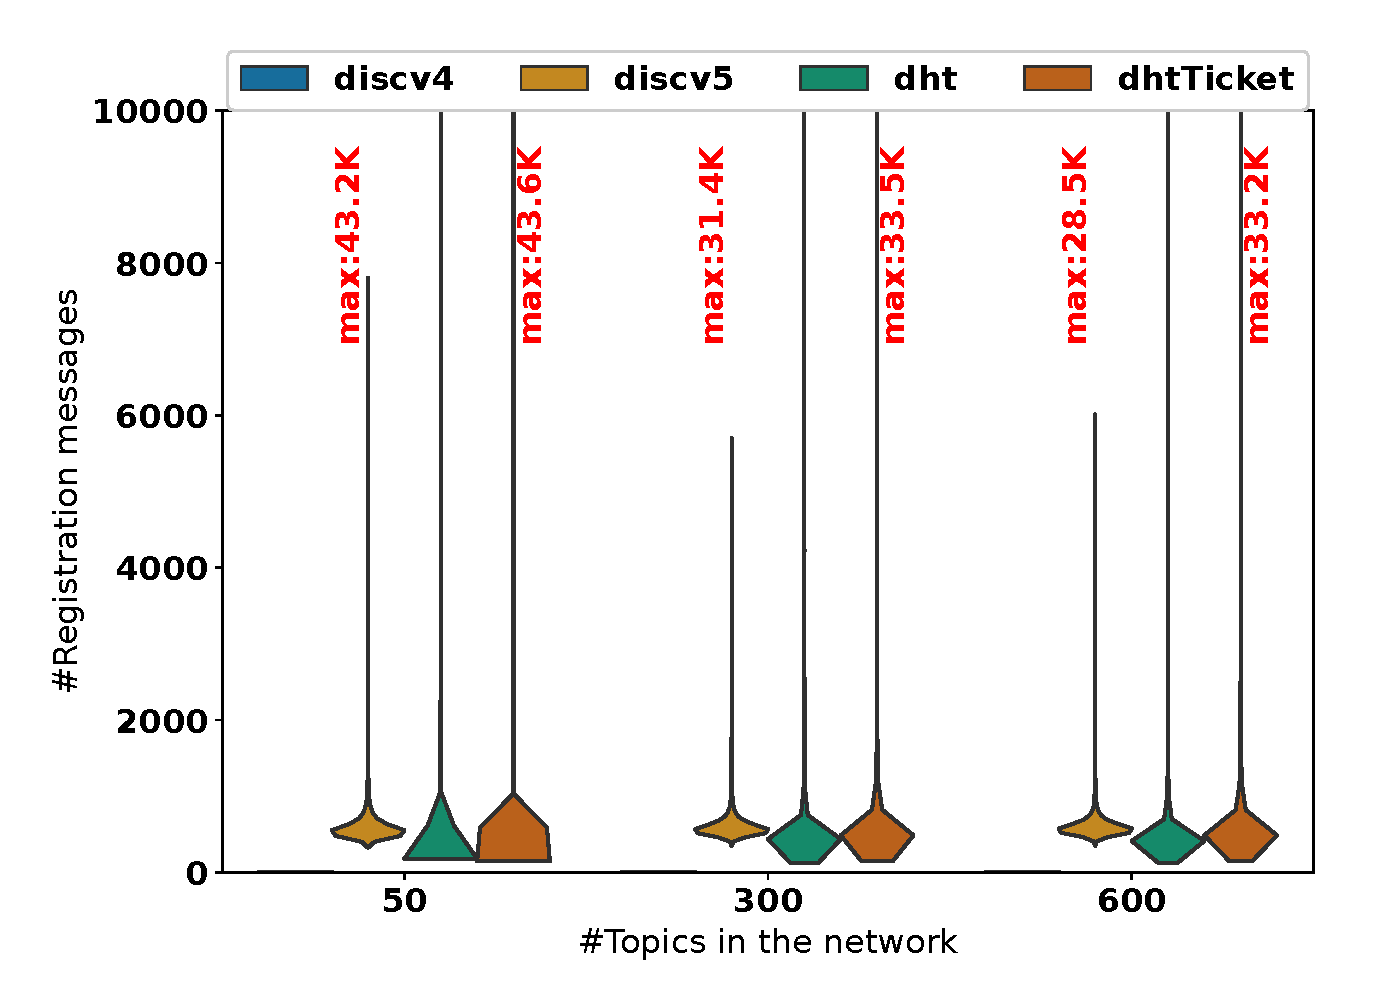
\includegraphics[width=\linewidth]{results/efficiency/violin_topic_registrationMsgs.eps}
%\caption{Y-axis: Distribution of registration related messages received by peers for varying number of topics for the simulation time.}
%\label{fig:regMsgsPerTopic}
%\end{figure}

%In~\Cref{fig:regMsgsPerTopic}~and~\Cref{fig:regMsgsPerSize},  we can observe while most of \sysname nodes receive around 500 registration messages,  with just a few receiving up to 5k messages in the worst case,  \altname solutions are more spread between 0 and 1000 received messages, but with some peaks up to 43k messages,  an order of magnitude higher than \sysname.
%This is caused by the fact that all nodes in \altname solutions try to put registrations starting by the closest nodes to the topic hash,  creating an uneven distribution  towards these nodes. 
%In \sysname, the use of \emph{advertise table} for advertisement placement provides a similar effect. 
%However this effect is diminished by the use of waiting times to regulate advertisement placement.  The increase of waiting time in the more congested nodes, causes that nodes starts more registrations in less congested nodes limiting the number of registrations placed on nodes close to topic hash.
%This effect is not seen when using \altname combined with tickets. 
%This is due to the fact that \altname is not using a \emph{advertise table} to keep track of ongoing registrations.  Because of this,  advertisers start new registrations towards the topic hash every advertisement period, even if they did not succeed in the previous attempts due to high waiting times.
%Therefore using tickets in the \altnameticket, maybe useful to increase the diversity in the \emph{advertise tables} but not for load balancing between nodes.
%
%When increasing the number of topics in the network (\Cref{fig:regMsgsPerTopic}), it is not observed an increase of registration messages for any of the different protocols. 
%However,  when increasing the number of nodes participating in the network (\Cref{fig:regMsgsPerSize}),  also registrations messages received per nodes are increased, as expected.
%But this increase is very different between \sysname and \altname protocols.
%\sr{tbc with specific values}

%\begin{figure}[!h]
%\centering
%\includegraphics[width=\linewidth]{results/split/size_registrationMsgs.eps}
%%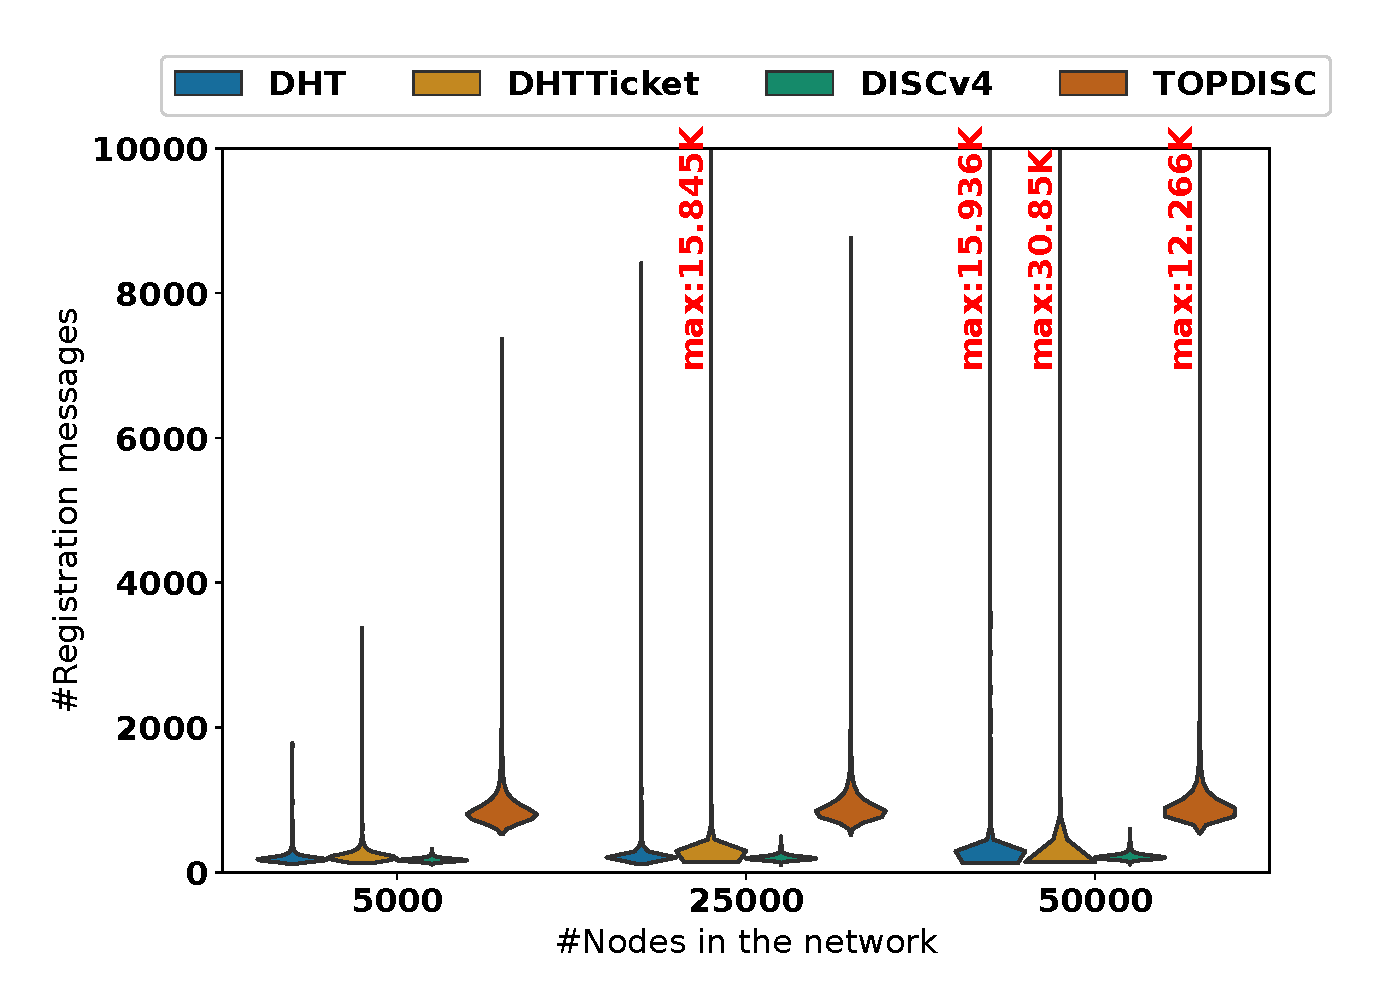
\includegraphics[width=\linewidth]{results/efficiency/violin_size_registrationMsgs.eps}
%\caption{Y-axis: Distribution of registration related messages received by peers for different network size for the simulation time.}
%\label{fig:regMsgsPerSize}
%\end{figure}
%
%\begin{figure}
%\centering
%\includegraphics[width=\linewidth]{results/split/topic_lookupMsgs.eps}
%%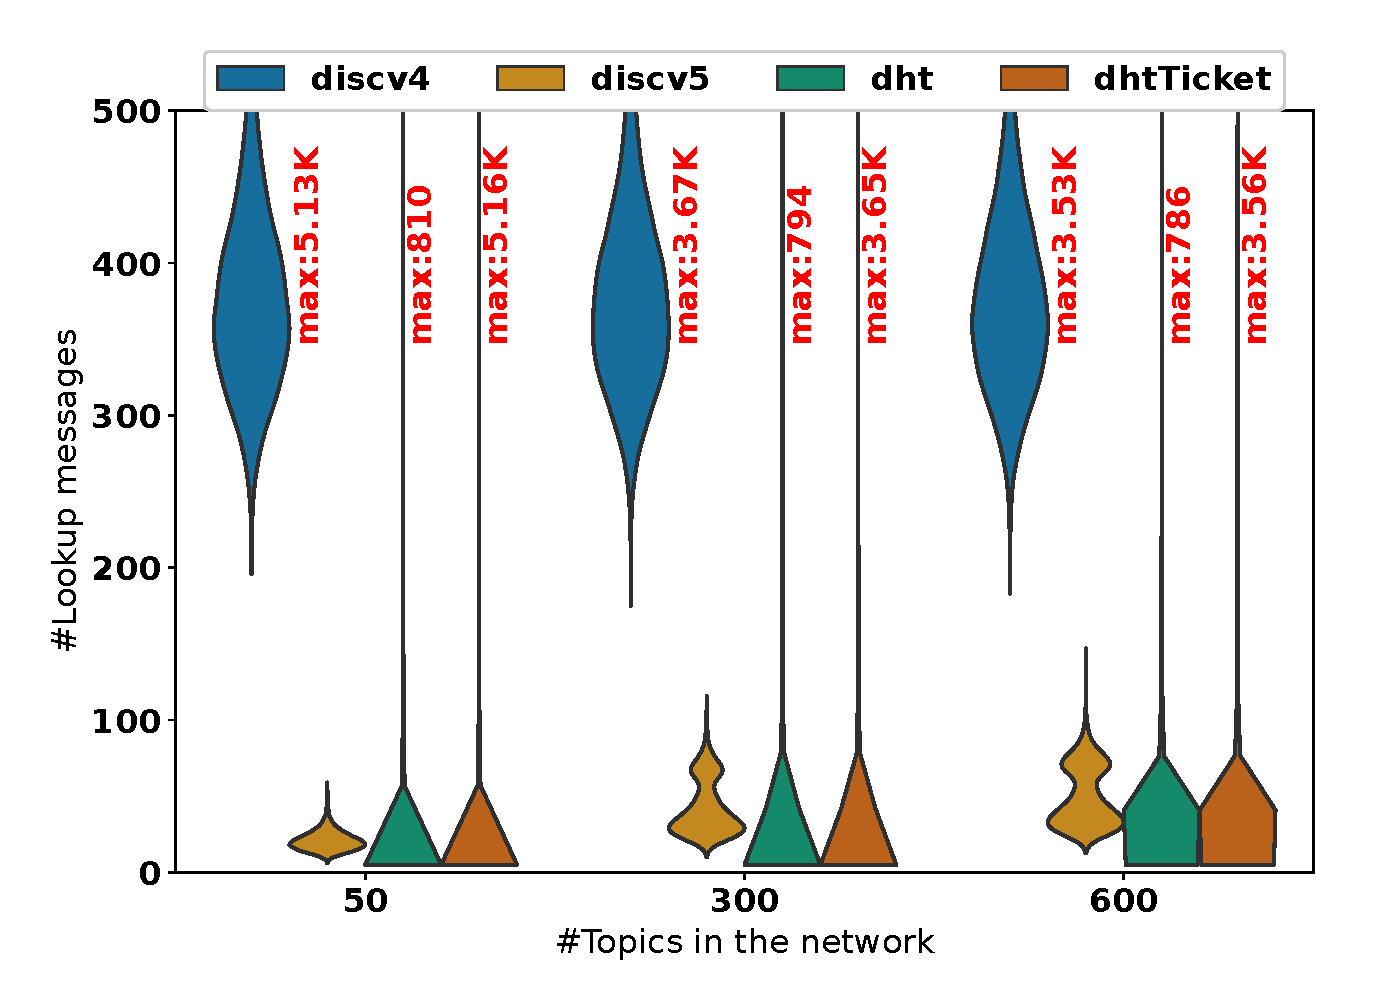
\includegraphics[width=\linewidth]{results/efficiency/violin_topic_lookupMsgs.eps}
%\caption{Y-axis: Distribution of lookup messages received by peers for varying number of topics for the simulation time.}
%\label{fig:lookupMsgPerTopic}
%\end{figure}
%
%\begin{figure}[!h]
%\centering
%\includegraphics[width=\linewidth]{results/split/size_lookupMsgs.eps}
%%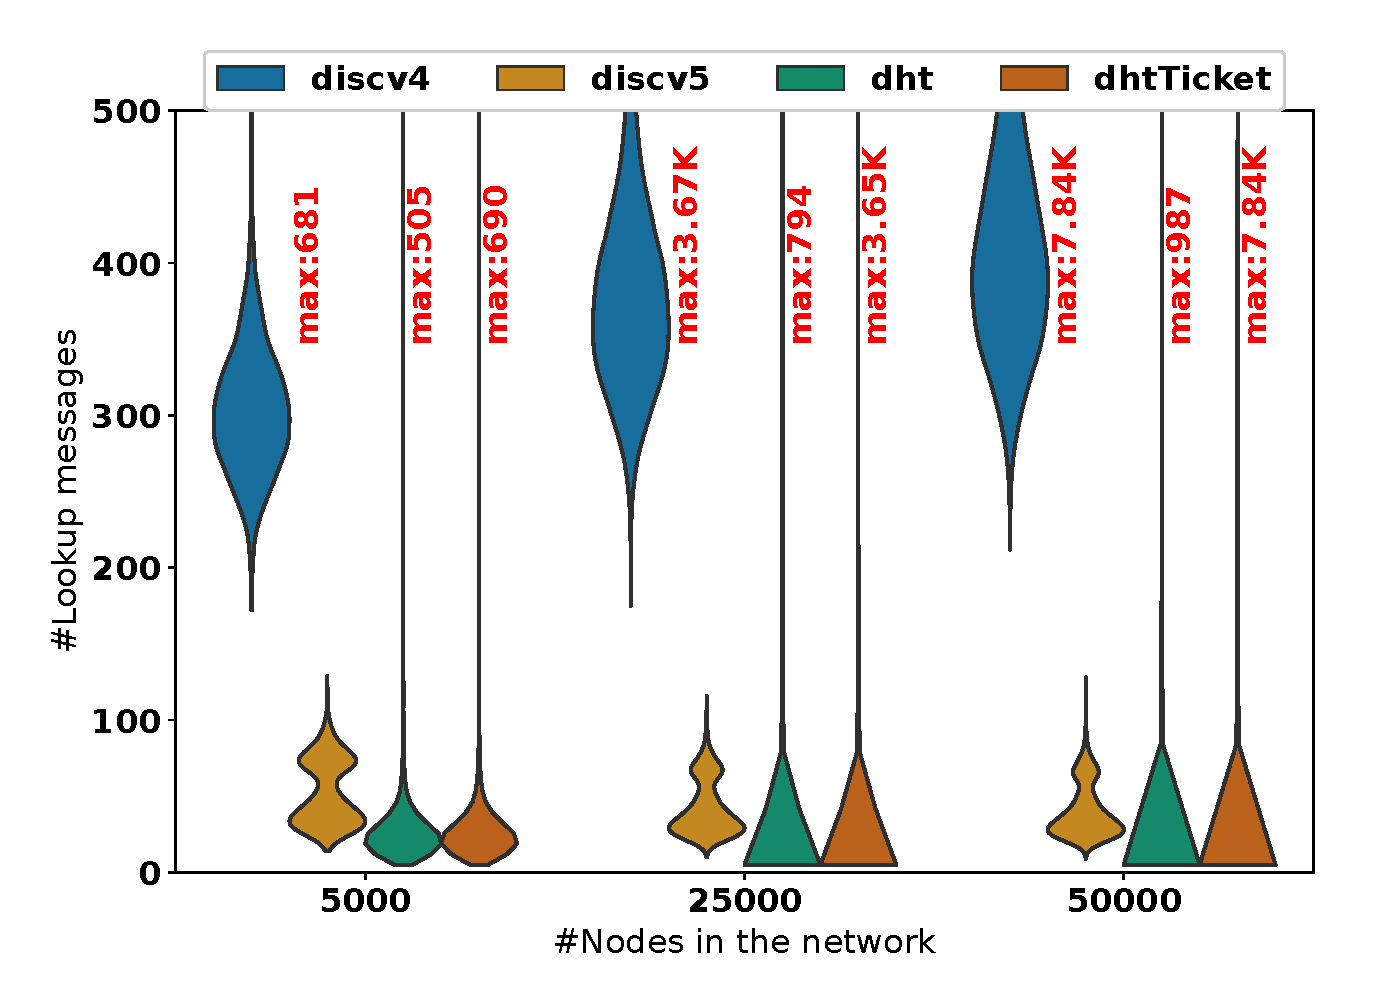
\includegraphics[width=\linewidth]{results/efficiency/violin_size_lookupMsgs.eps}
%\caption{Y-axis: Distribution of lookup messages received by peers for different network size for the simulation time.}
%\label{fig:lookupMsgPerSize}
%\end{figure}

%In~\Cref{fig:lookupMsgPerTopic}~and~\Cref{fig:lookupMsgPerSize}, we observe the number of messages related to the lookup process, \ie topic queries and replies for \sysname, \altname and \altnameticket, and kademlia find/response messages for \discv. We evaluated using  different network sizes and different number of topics in the network. 
%There is a single lookup in the simulation per node, and the $N_\textit{lookup}$ parameter used is equal to 30.  Therefore nodes stop the lookup process when found 30 different nodes in the network for the intended topic.
%In the figures we can observe there is a big different between topic-aware protocols (\sysname, \altname and \altnameticket) and \discv. 
%
%\sr{why there is an increase for \discv with the number of nodes in the simulation and not the number of topics??? shouldn't be the opposite? I guess is because even if there are topics with less nodes there is just a single lookup with the same nodes contacted}
%\sr{why the peak is bigger for DHT for 600 than 300? Is it because of topic hash ids colliding?}

\begin{figure}[!h]
\centering
\includegraphics[width=\linewidth]{results/split/size_totalMsg.eps}
%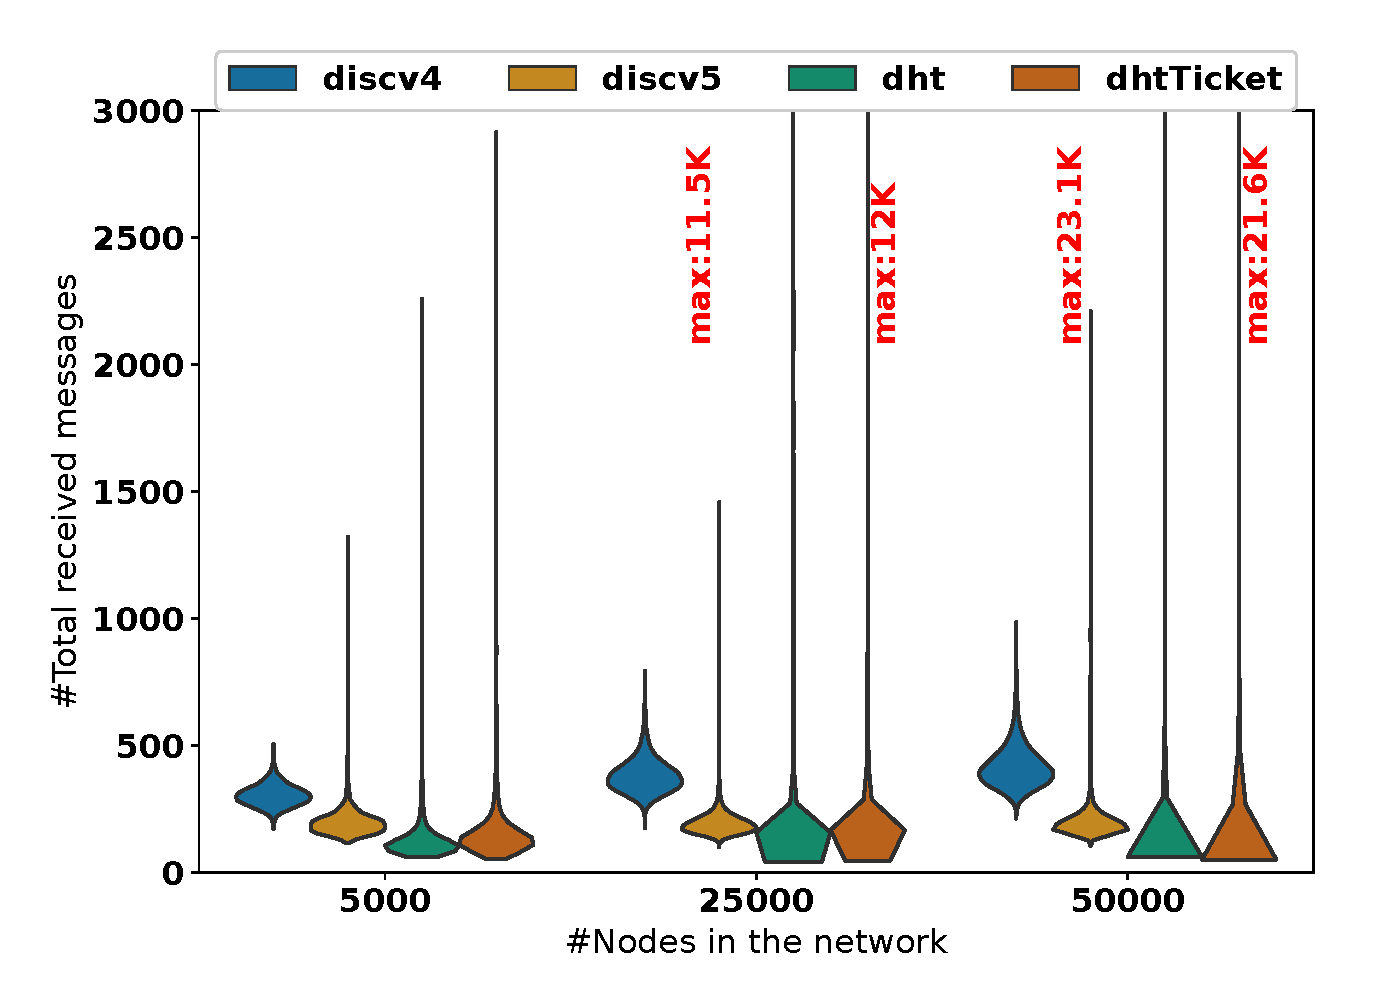
\includegraphics[width=\linewidth]{results/efficiency/violin_size_totalMsg.eps}
\caption{Y-axis: Distribution of discovery related (including registration and lookup) messages received by peers for different network size during a single advertisement period.}
\label{fig:msgsPerSize}
\end{figure}

\begin{figure}
\centering
\includegraphics[width=\linewidth]{results/split/topic_totalMsg.eps}
%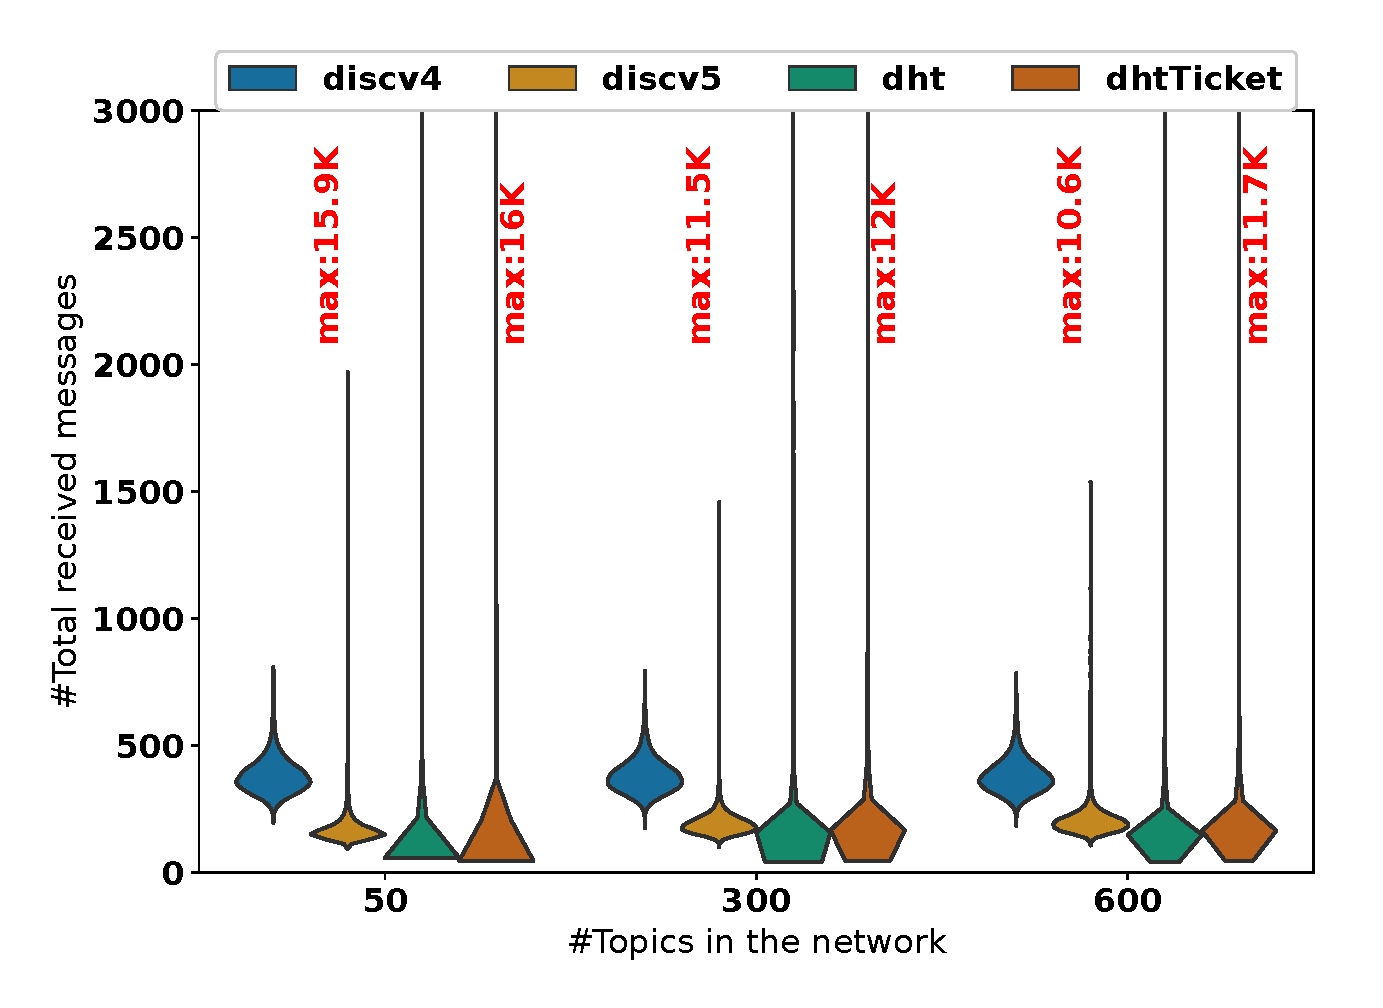
\includegraphics[width=\linewidth]{results/efficiency/violin_topic_totalMsg.eps}
\caption{Y-axis: Distribution of discovery related (including registration and lookup) messages received by peers for different number of topics during a single advertisement period.}
\label{fig:msgsPerTopic}
\end{figure}

In~\Cref{fig:msgsPerSize}~and~\Cref{fig:msgsPerTopic}, we observe the total number of messages during the simulation but normalised per advertisement period. 
Therefore in the figures, it is shown the messages related to a single lookup per node and a single registration process per node before advertisements start to expire and need to be refreshed.
This the overall overhead registered per node in the network.
We can observe that \altname protocols does not scale with the increase of nodes in the network. 
Nodes that are close to a topic hash receive most of the traffic and there is a linear increase with the number of nodes in the network. 
\discv protocol has a better distribution of the load between nodes since its behaviour is completely random. However, the average load in nodes is the highest one because of the overhead caused by not being able to find nodes for specific topics, increasing the overhead during lookup.
\sysname in comparison, provides lower overhead than the other protocols.

%%%%%%%%%%%%%%%%%%%%%%%%%%%%%%%%%%%%%%%%%%%%%%%%%%%%%%%%%%%
\subsection{Lookup performance}

\begin{figure}[!h]
\includegraphics[width=\linewidth]{results/split/topic_discovered.eps}
%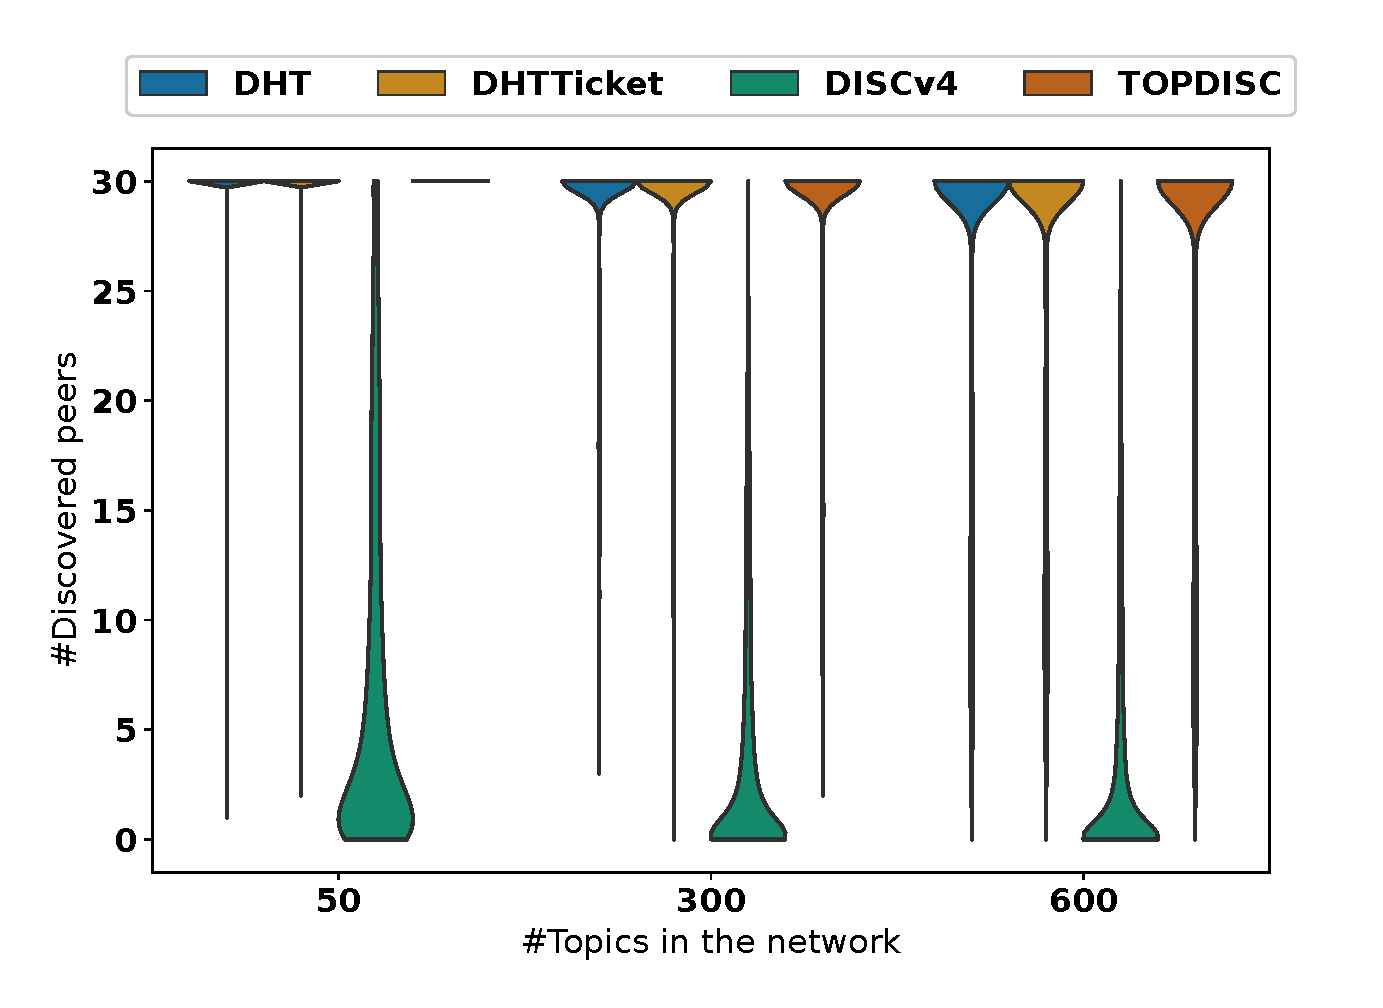
\includegraphics[width=\linewidth]{results/efficiency/violin_topic_discovered.eps}
\caption{Y-axis: Distribution of the number of peers discovered during lookup operation for different number of topics.}
\label{fig:discoveredPerTopic}
\end{figure}

\Cref{fig:discoveredPerTopic} presents the number of peers discovered during a single lookup operation with increasing number of topics in the network. The discovery becomes more difficult, as the number of topics grows.  \discv achieves a much lower number of discovered peers per operation, while \sysname and DHT-based solution efficiently discover the required amount of nodes. The rare cases where \sysname and DHT-based solution do not discover the required amount of peers are caused by small networks that consist of less than 30 nodes. 

\michal{regarding \Cref{fig:discoveredPerTopic}, it seems that for 300 and 600 topics, we discover slightly less peers on average than the DHT solutions. Why is that? Those results should be for the same topic distributions across protocols, right?}
\sergi{I think is normal and is caused by the fact that dht is going straight to nodes with most of the registrations so, specially with topics with very few nodes, they can find nodes faster, but with the tradeoff of being eclipsed very easy.}

\begin{figure}[!h]
\includegraphics[width=\linewidth]{results/split/size_discovered.eps}
%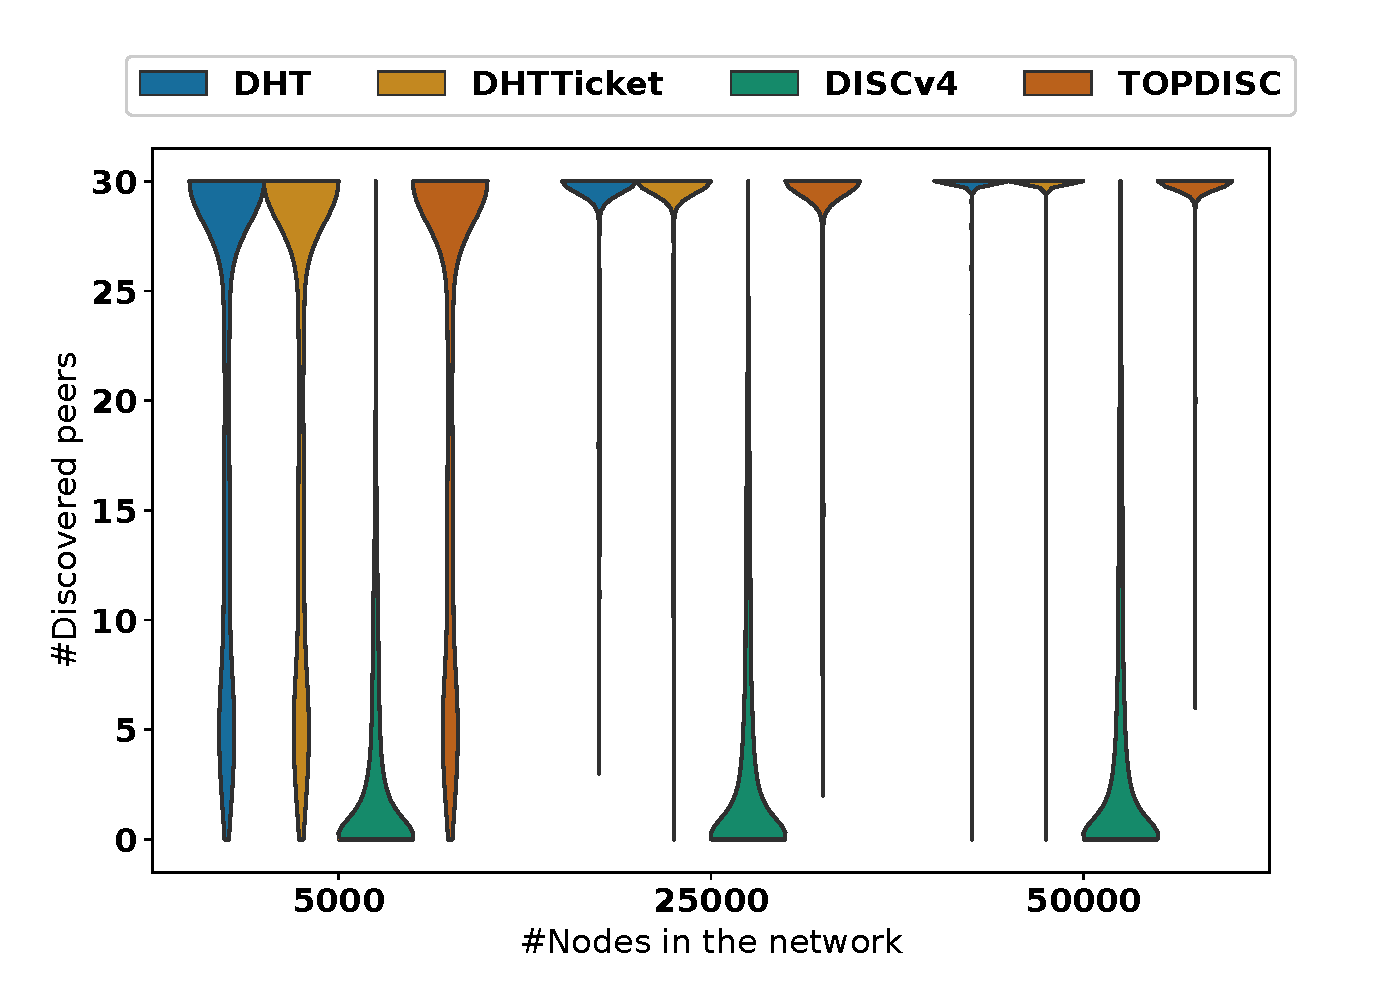
\includegraphics[width=\linewidth]{results/efficiency/violin_size_discovered.eps}
\caption{Y-axis: Distribution of the number of peers discovered during lookup operation for different network size.}
\label{fig:discoveredPerSize}
\end{figure}

\Cref{fig:discoveredPerSize} presents the number of peers discovered during a single lookup operation with increasing size of the network. With a fixed amount of topics, each application-specific network grows and for all the protocols, it is easier to find the required amount of nodes. However, discv4 suffers from poor performance for all the investigated network sizes. 

\begin{figure}
\includegraphics[width=\linewidth]{results/split/topic_wasDiscovered.eps}
%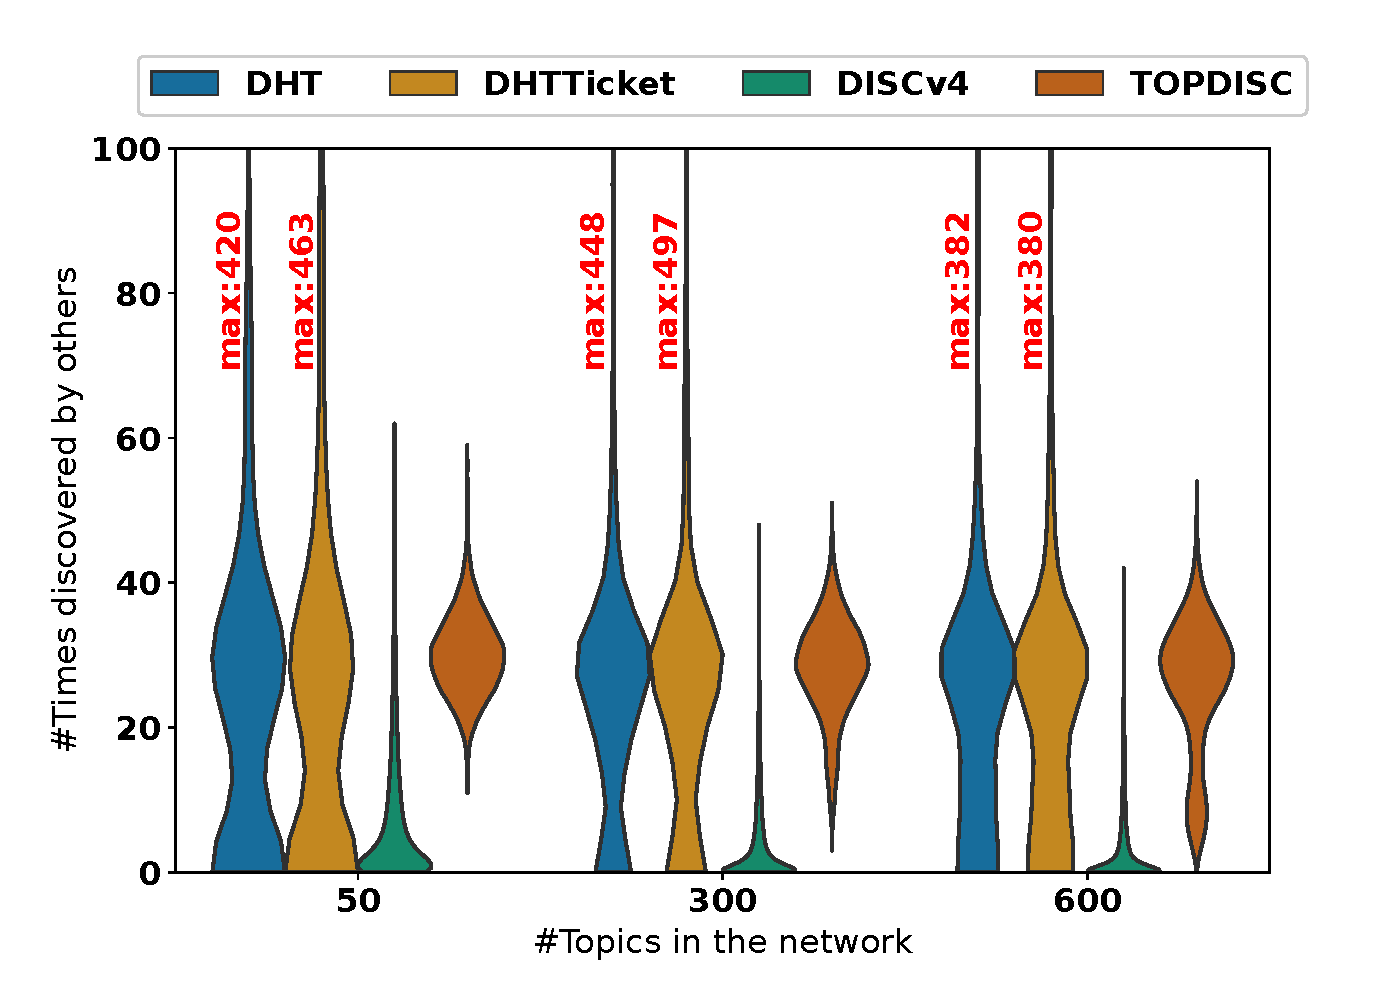
\includegraphics[width=\linewidth]{results/efficiency/violin_topic_wasDiscovered.eps}
\caption{Y-axis: Distribution of the number of times a peer is discovered by others for number of topics in the network for the simulation time.}
\label{fig:discoveredByPerTopic}
\end{figure}

\begin{figure}[!h]
\includegraphics[width=\linewidth]{results/split/size_wasDiscovered.eps}
%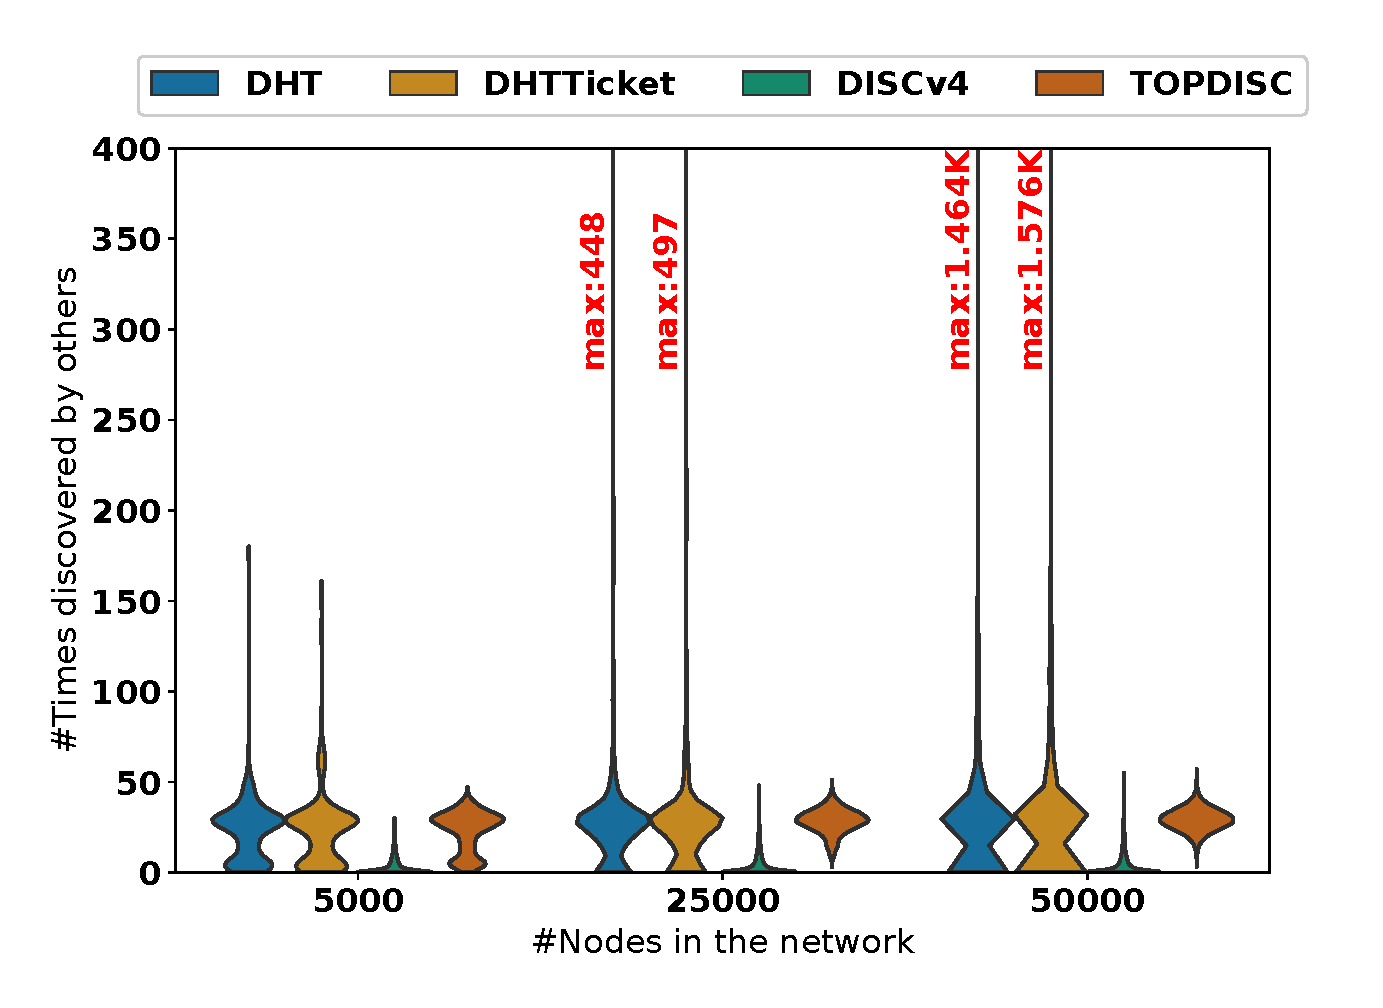
\includegraphics[width=\linewidth]{results/efficiency/violin_size_wasDiscovered.eps}
\caption{Y-axis: Distribution of the number of times a peer is discovered by others for different network size for the simulation time.}
\label{fig:efficiency_size}
\end{figure}

%\subsection{Registrations}
%
%
%\begin{figure}
%\includegraphics[width=\linewidth]{results/split/topic_regsPlaced.eps}
%%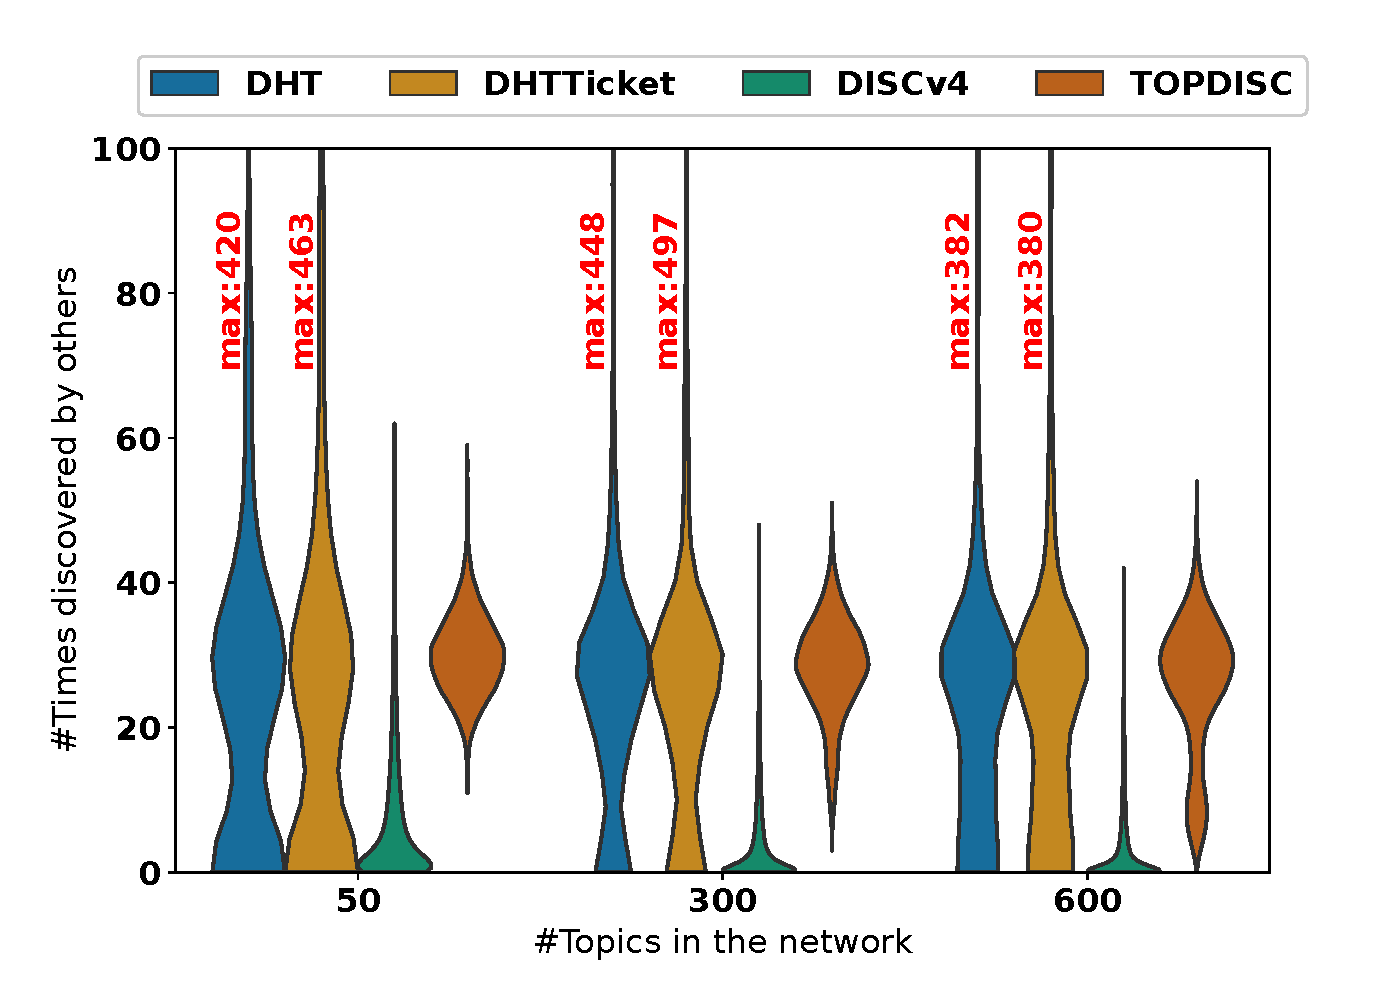
\includegraphics[width=\linewidth]{results/efficiency/violin_topic_wasDiscovered.eps}
%\caption{Y-axis: .}
%\label{fig:regsPlacedPerTopic}
%\end{figure}
%
%\begin{figure}[!h]
%\includegraphics[width=\linewidth]{results/split/size_regsPlaced.eps}
%%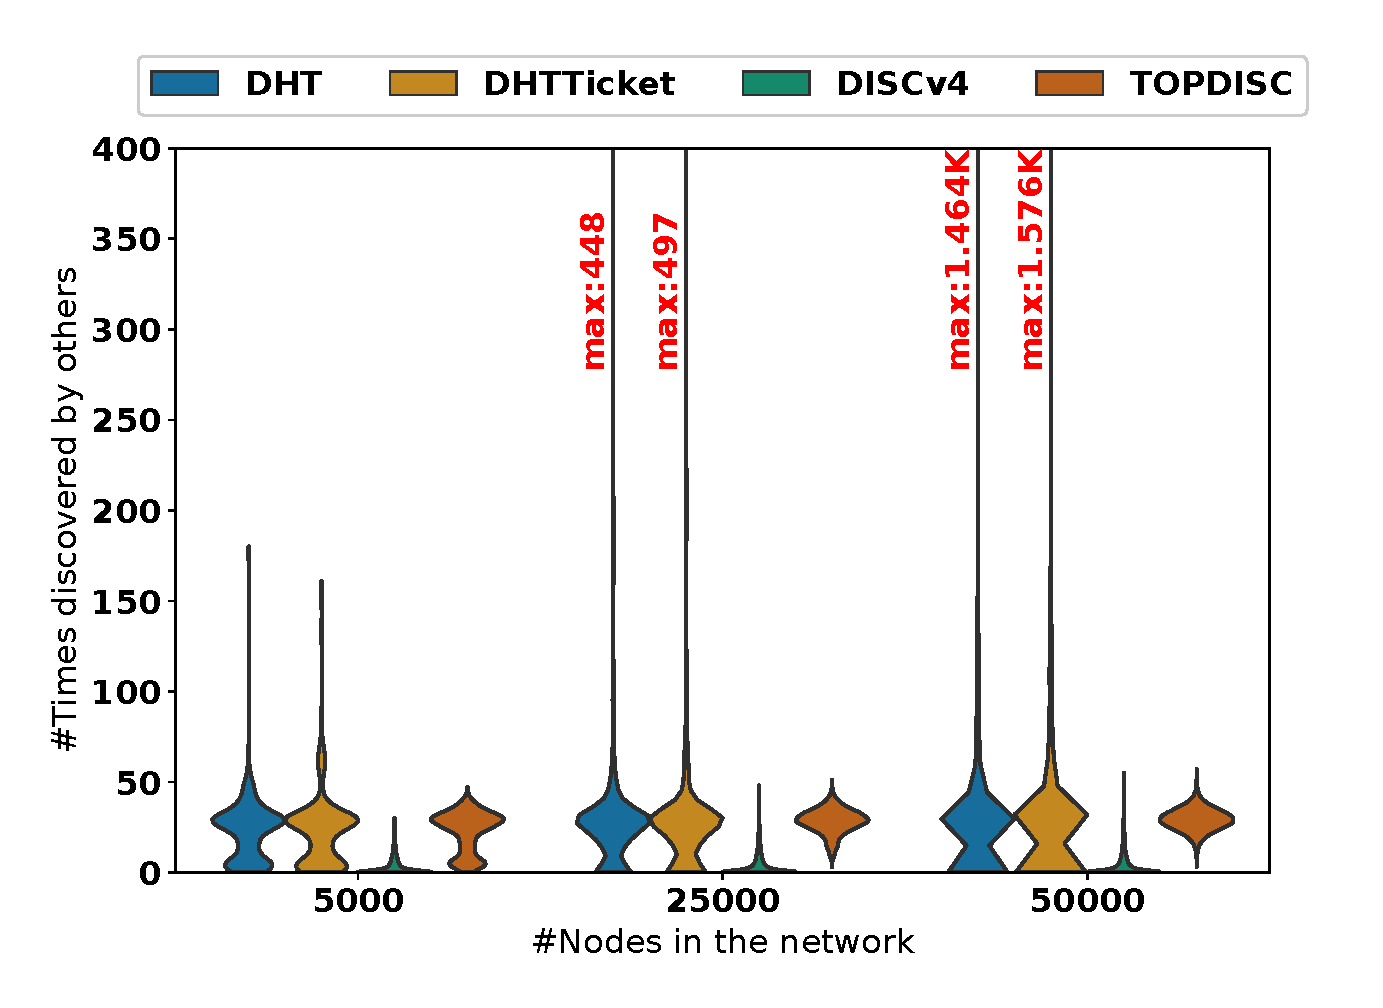
\includegraphics[width=\linewidth]{results/efficiency/violin_size_wasDiscovered.eps}
%\caption{Y-axis: .}
%\label{fig:regsPlacedPerSize}
%\end{figure}
%
%\begin{figure}
%\includegraphics[width=\linewidth]{results/split/topic_regsAccepted.eps}
%%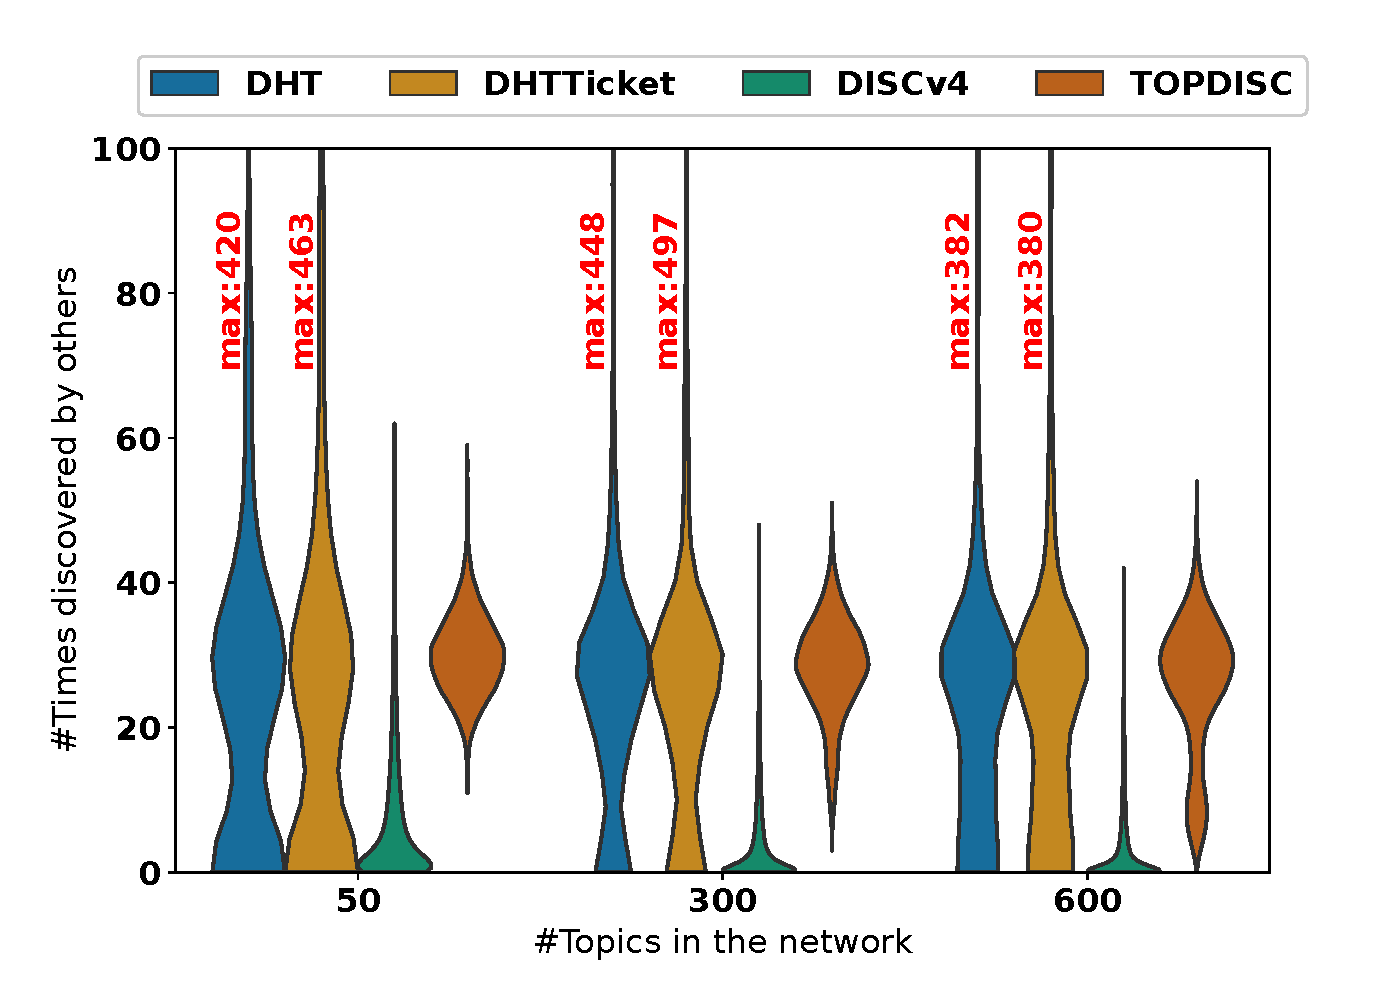
\includegraphics[width=\linewidth]{results/efficiency/violin_topic_wasDiscovered.eps}
%\caption{Y-axis: .}
%\label{fig:regsAcceptedTopic}
%\end{figure}
%
%\begin{figure}[!h]
%\includegraphics[width=\linewidth]{results/split/size_regsAccepted.eps}
%%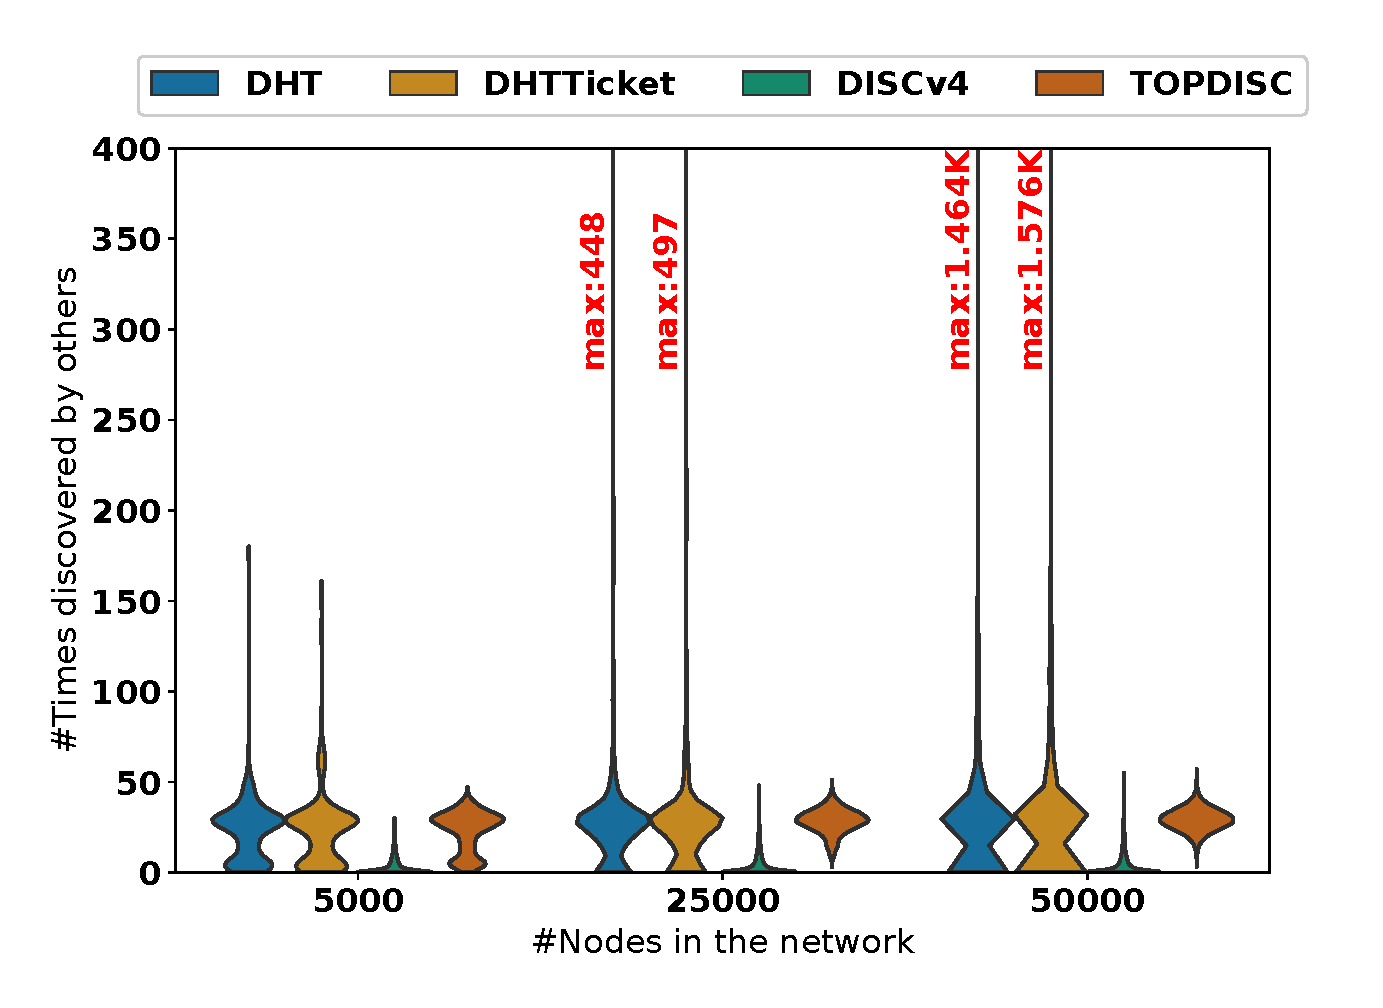
\includegraphics[width=\linewidth]{results/efficiency/violin_size_wasDiscovered.eps}
%\caption{Y-axis: .}
%\label{fig:regsAcceptedSize}
%\end{figure}

\subsection{Security}
%We evaluate \sysname resistance to two groups of malicious attacks:
%\begin{itemize}
%    \item \textbf{Eclipse Attack} - the attacker tries to make a target node discover and connect to peers under the attacker's control. The attack succeeds when all the inbound and outbound connections of the target node are established with malicious peers. 
%    \item \textbf{Denial of Service (DoS)} - the attacker tries to disturb protocol operations. The attack succeeds when service discovery is made impossible or significantly delayed for a group of benign nodes.  
%\end{itemize}
%The attacker may use a large but finite number of malicious nodes. Both attacks may target a single node or a group of nodes (\eg nodes participating in a specific application). 

%\para{Eclipse Attack}

\para{Eclipse Attack}
We implemented and evaluated \sysname resistance against a hybrid eclipse attack targeted to a specific topic,  that  tries to make a searcher node discover and connect to peers under the attacker's control.  
The attacker may be able to generate a large but finite number of Sybil nodes,  with limited network resources (\ie limited IP addresses used by the Sybil nodes pool used in the attack).
The attack succeeds when all the inbound and outbound connections of the target node are established with malicious peers.  The attack consists of the following:
\begin{itemize}
    \item \textbf{Registration spam} - the attacker targets a registrars and sends a large number of registrations requests. If successful, the attacker exhaust registrar's resources and prevent benign nodes from registering. 
%    \item \textbf{Malicious registrar} - the attacker deploys its nodes playing the role of registrars that \textit{(i)} return maximum waiting times when asked for a ticket, \textit{(ii)} return an empty set when asked about a topic. If successful, the attacker prevents benign advertisers from registering \textit{(i)} and prevents benign searchers from discovering their peers \textit{(ii)}. 
	\item \textbf{Malicious registrar} - the attacker deploys its nodes playing the role of registrars that only malicious sybils with the objective of preventing benign searchers from discovering valid peers and eclipsing all its connections.  We consider a coordinated eclipsing attack and any malicious registrar replies with a subset of the identifiers of the Sybil nodes controlled by the attacker.
\end{itemize}

We evaluated the resistance against eclipse attacks using the same default parameters used in the performance evaluation, that is 25000 nodes in the simulation and 300 topics by default, distributed using zipf function of exponent 1.0.  The simulation runs for 1 hour and there is a single lookup per node for the topic it participates.
Nodes get eclipsed when all nodes discovered during a lookup are malicious nodes controlled by the attacker, and therefore they only can connect to the attacker and get the view of the network from the attacker only. 

In the following figures we show violin plots representing the number of malicious nodes returned per lookup using different parameters for the same protocols evaluated in the performance simulations.  On top of each violin plot we specify the percentage of nodes eclipsed after a lookup (\ie percentage of lookups where all nodes returned are malicious nodes).
We evaluated the eclipse attacks targeting two specific topis, the most popular topic and a low popularity topic.
The most popular topic has 3978 nodes registering for this topic and the low popularity has only 33 nodes.
We evaluated the attacks for the most popular and least popular 


\begin{figure}[!h]
\includegraphics[width=\linewidth]{results/security/violin_idDistribution_percentageMaliciousDiscovered_t0.eps}
\caption{Y-axis: Malicious nodes discovered and percentage eclipsed nodes using uniform distributed sybil identities vs generating node ids close to topic id,   when attacking the most popular topic (3978 nodes).}
\label{fig:eclipse_distribution_t0}
\end{figure}

In Figure~\ref{fig:eclipse_distribution_t0} we show the malicious nodes discovered for all lookups for all protocols using different distribution of the identifiers of the malicious nodes,  when attacking the most popular topic (with 3978 nodes).  In the first option, the malicious nodes ids are artificially generated with a small distance to the topic hash id.  In the second option, malicious nodes identifiers are uniformly distributed.  In the figure we can observe that for \altname and \altnameticket the percentage of eclipses are superior to 80\% because most of the nodes close to topics identifiers are nodes controlled by the attacker.  
For \altname and \altnameticket, the lookup process is similar to Kademlia lookup process and,  placing all malicious nodes close the topic hash,  it makes very likely to query only malicious nodes during the process, since it only queries the closest known nodes to the topic identifier.
When attackers are uniformly distributed in the network, eclipses are reduced to close to 32.9\% and 33.7\% respectively.
Even though it is much less likely to hit malicious nodes during the lookup in this case (remember the default number of malicious are 1000 -4\% of the network-),  when hitting a malicious nodes, the nodes returned by them are used to continue the  query and it may happen it continues querying malicious nodes only during the process.
When a low popularity topic is attacked (with only 33 nodes),  as shown in Figure~\ref{fig:eclipse_distribution_t299},  for  \altname and \altnameticket the eclipses are even higher, reaching a 100\% of eclipses when placing malicious nodes close to the topic id, and reaching a 78.8\% and 90.9\% when distributing malicious nodes uniformly.  
Remember the number of attackers is 1000,  against the 33 valid nodes.

For \discv,  the number of eclipses reach is 0\% for the most popular topic when attackers are placed close to the topic hash.  When Sybil nodes are uniformly distributed the number of malicious nodes returned increases,  but to a very low 0.1\%.
This is caused by the fact that \discv does not target lookups to any specific identifier,  but completely random identifiers,  so it is very difficult for the attackers to place Sybil nodes where they will be queried.  Moreover it is difficult by the attackers to send identifiers where the lookup process will be likely to continue to,  because in the FIND node for the Ethereum DHT the lookup identifier is not disclosed,  but only the distance to it.
The number of eclipses reach 12.1.\% for the least popular topic when attackers are placed close to the topic hash.  When Sybil nodes are uniformly distributed the number of malicious nodes returned increases,  however the eclipses  reach a 78.8\%.
The resistance of \discv to Sybil attacks is obtained with the important trade-off of very low efficiency when finding nodes for specific topics, specially for low popular topics.  It is very likely that, when doing lookups using \discv for very low popular topics, no nodes are found or just a few of them.   This means when hitting a malicious node during lookup,  it is likely with a single query to a malicious node, the node querying will be eclipsed.

For \sysname, the number of eclipses are very low for the most popular topic. 
The eclipses are 0\% when Sybil nodes are placed close to topic id and 0.5\% when are uniformly distributed, with similar distribution to the malicious nodes returned compared with \discv.
However when attacking the least popular topic the eclipses increase to 78.8\% for both cases.
This is due to the very low number of valid nodes (33),  that will be more difficult to find than the attackers (1000 nodes, reusing 100 IP addresses).  
But event the high number of attackers in almost half the cases valid nodes are also found along the evil nodes.
Remember that Sybil nodes are completely valid nodes from a network discovery point of view when using different network addresses.

\begin{figure}[!h]
\includegraphics[width=\linewidth]{results/security/violin_idDistribution_percentageMaliciousDiscovered_t299.eps}
\caption{Y-axis: Malicious nodes discovered and percentage eclipsed nodes using uniform distributed sybil identities vs generating node ids close to topic id,   when attacking the low popularity topic (33 nodes).}
\label{fig:eclipse_distribution_t299}
\end{figure}

In Figure~\ref{fig:eclipse_evil_t0} we show the malicious nodes discovered for all lookups for all protocols, using different number of Sybil nodes in the network,  when attacking the most popular topic,  and in Figure~\ref{fig:eclipse_evil_t299} we show the malicious nodes discovered for the least popular topic.  In both figures attackers identifiers are generated uniformly and attackers use a pool of 100 IP addresses. 
In Figure~\ref{fig:eclipse_evil_t0}, we observe \discv is the protocol with the lowest number of eclipses and with the best distribution of malicious nodes returned during lookups.  However \sysname performs very close to \discv, having only 0.2\% of eclipses when there are 1000 attackers in the network.
\altname and \altnameticket has the worst performance,  having 47.7\% and 48.4\% of eclipses when when there are 2500 attackers.
In Figure~\ref{fig:eclipse_evil_t299}, when attacking least popular topic, we observe \sysname is the most resistant to eclipsing.
This is because it is the protocol that is able to discover more nodes with a higher diversity and is the protocol that will find easier the any of the few valid nodes in the network, and therefore it will be not eclipsed.
 
\begin{figure}[!h]
\includegraphics[width=\linewidth]{results/security/violin_percentEvil_percentageMaliciousDiscovered_t0.eps}
\caption{Y-axis: Malicious nodes discovered and percentage eclipsed nodes for different number of sybil nodes used in the attack,  when attacking the most popular topic (3978 nodes).}
\label{fig:eclipse_evil_t0}
\end{figure}

\begin{figure}[!h]
\includegraphics[width=\linewidth]{results/security/violin_percentEvil_percentageMaliciousDiscovered_t299.eps}
\caption{Y-axis: Malicious nodes discovered and percentage eclipsed nodes for different number of sybil nodes used in the attack,  when attacking the low popularity topic (33 nodes).}
\label{fig:eclipse_evil_t299}
\end{figure}


In Figure~\ref{fig:eclipse_sybil_t0} we show the malicious nodes discovered for different number of IP addresses available to the attacker,  when attacking the most popular topic,  and in Figure~\ref{fig:eclipse_sybil_t299} we show the malicious nodes discovered when attacking the least popular topic.
In this case we observe the same results than for the default values. 
\sysname is very close to \discv performance with eclipses closes to 0\% for the most popular topic, and \altname and \altnameticket is close to 33\% eclipses in all cases.
When attacking the low popularity topic,  nodes eclipsed are very similar but having a slight better performance \discv and \sysname.
There is not appreciated in the results any effect of increasing the number of IPs used by the attackers for any of the protocols.
This is caused by the fact that what is more important for the eclipses is whether you hit a malicious node during the lookup process rather than the registrations attackers are able to place in other nodes.

\begin{figure}[!h]
\includegraphics[width=\linewidth]{results/security/violin_sybilSize_percentageMaliciousDiscovered_t0.eps}
\caption{Y-axis: Malicious nodes discovered and percentage eclipsed nodes for different number IP addresses used in the attack,  when attacking the most popular topic (3978 nodes).}
\label{fig:eclipse_sybil_t0}
\end{figure}



\begin{figure}[!h]
\includegraphics[width=\linewidth]{results/security/violin_sybilSize_percentageMaliciousDiscovered_t299.eps}
\caption{Y-axis: Malicious nodes discovered and percentage eclipsed nodes for different number IP addresses used in the attack,  when attacking the least popular topic (33 nodes).}
\label{fig:eclipse_sybil_t299}
\end{figure}



%\begin{figure*}[!h]
%\centering
%\subfigure[{Y-axis: Percentage eclipsed nodes using uniform distributed sybil identities vs generating node ids close to topic id}]{
%\includegraphics[width=0.31\textwidth]{results/security/%bar_idDistribution_percentageEclipsedLookups_t0.eps}
%violin_idDistribution_percentageMaliciousDiscovered_t0.eps}
%\label{fig:distribution}
%}
%\subfigure[{Y-axis: Percentage eclipsed nodes for different number of sybil nodes in the attack.}]{
%\includegraphics[width=0.31\linewidth]{results/security/%bar_percentEvil_percentageEclipsedLookups_t0.eps}
%violin_percentEvil_percentageMaliciousDiscovered_t0.eps}
%\label{fig:percentEvil}
%}
%\subfigure[{Y-axis: Percentage eclipsed nodes for different number IP addresses used in the attack.}]{
%\includegraphics[width=0.31\linewidth]{results/security/%bar_sybilSize_percentageEclipsedLookups_t0.eps}
%violin_sybilSize_percentageMaliciousDiscovered_t0.eps}
%\label{fig:sybilsize}
%}
%\caption{Resistance against eclipse attacks when attacking most popular topic (t0)} 
%\label{fig:eclipse_attack}
%\vspace{-0.05in}
%\end{figure*}
%
%\begin{figure*}[!h]
%\centering
%\subfigure[{Y-axis: Percentage eclipsed nodes using uniform distributed sybil identities vs generating node ids close to topic id}]{
%\includegraphics[width=0.31\textwidth]{results/security/%bar_idDistribution_percentageEclipsedLookups_t299.eps}
%violin_idDistribution_percentageMaliciousDiscovered_t299.eps}
%\label{fig:distribution}
%}
%\subfigure[{Y-axis: Percentage eclipsed nodes for different number of sybil nodes in the attack.}]{
%\includegraphics[width=0.31\linewidth]{results/security/%bar_percentEvil_percentageEclipsedLookups_t299.eps}
%violin_percentEvil_percentageMaliciousDiscovered_t299.eps}
%\label{fig:percentEvil}
%}
%\subfigure[{Y-axis: Percentage eclipsed nodes for different number IP addresses used in the attack.}]{
%\includegraphics[width=0.31\linewidth]{results/security/%bar_sybilSize_percentageEclipsedLookups_t299.eps}
%violin_sybilSize_percentageMaliciousDiscovered_t299.eps}
%\label{fig:sybilsize}
%}
%\caption{Resistance against eclipse attacks when attacking least popular topic (t299)} 
%\label{fig:eclipse_attack}
%\vspace{-0.05in}
%\end{figure*}
%\begin{figure}[!h]
%
\includegraphics[width=\linewidth]{img/placeholder}
%\caption{Compare only against DHT here I guess? Y-axis a ratio of popular malicious and benign ads in the table for spam attack and topic-targeted attack within a single registrar. X-axis: to avoid showing different graphs for multiple malicious IPs/IDs/nodes we can have a fix ratio between them i.e., each 5 Sybils (or requests/s) have 1 IP and 2 ID, and increase this "attacker strength".} 
%\label{fig:security_spam}
%\end{figure}
%
%\begin{figure}[!h]
%
\includegraphics[width=\linewidth]{img/placeholder}
%\caption{Compare only against DHT here I guess? Y-axis a  time to discovery/registration (do we care about registration if lookup works?) slowdown compared to a non-attack scenario?Do we consider different placements of Sybils here (i.e., only bucket 1? Or spread evenly across all the buckets?). X-axis: to avoid showing different graphs for multiple malicious IPs/IDs/nodes we can have a fix ratio between them i.e., each 5 Sybils have 1 IP and 2 ID, and increase this "attacker strength".} 
%\label{fig:security_spam}
%\end{figure}



\iffalse
\subsection{Performance Results}
\michal{We should group the result so that they show achievement of specific goals that we described before}

%\paragraph{Ticket registrations:
In the following we detail the performance evaluation in four different subsections.  In the first we show the registration performance.  Secondly we show the traffic load and overhead of the designed mechanism.  Then we continue with the lookup and discovery performance and we finish with the security analysis.

\subsubsection{Registration  performance}

In Figure~\ref{fig:regs} we observe the average active registrations in the system per topic with different number of nodes in the simulation,  from 500 to 10000 nodes. 
We can observe nodes for all topics are able to place a substantial amount of registrations, even the less popular topics. 
As number of nodes increase in the network, we can observe the differences between registrations per topic are reduced. 
Actually, it can be observed the most popular topic (t1) is able to place less registrations than t2. 
This is caused by the fact that with more nodes trying to register for the same topic,  waiting times increase.
If the waiting time increases over the waiting time limit (in the simulations is set to 15 min),  the node cancels the registration and tries with a different nodes.
When cancellations happen it may lead to less active registrations, because it may end up with longer registration processes.
In our simulation we observe less registrations for t1 than t2  because t1 registrations waiting time go over the waiting time limit more often.

In Figure~\ref{fig:time_reg} we observe the average time necessary for a node to place a registration,  from 500 to 10000 nodes in the simulation.
We can observe that average registration time is always below 500 seconds and this is reduced for less popular topics and smaller networks. 
This figure does not include registration times for cancelled registrations.
\sergi{I think we should include failed/uncomplete registrations in the plot}

\begin{figure}[!h]
\centering
\subfigure[{Active registrations}]{
\includegraphics[width=0.225\textwidth]{img/eval/registration_origin.eps}
\label{fig:regs}
} 
\hspace{-0.25cm}
\subfigure[{Time to register}]{
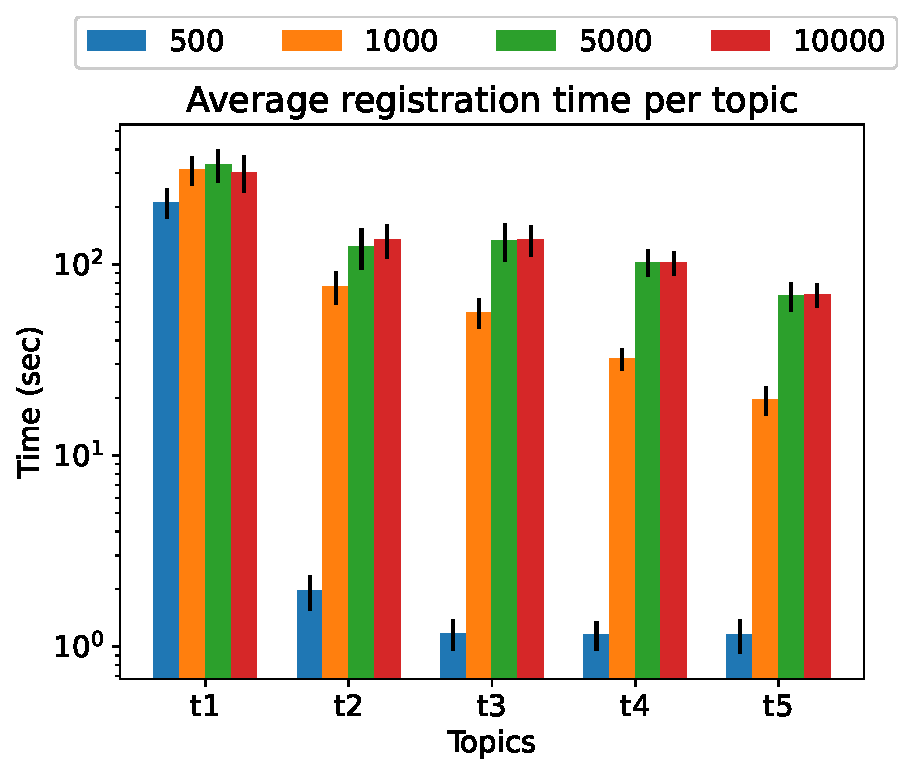
\includegraphics[width=0.225\textwidth]{img/eval/avg_time_register.eps}
\label{fig:time_reg}
}
 \caption{Ticket registrations} 
\label{fig:registrations}
\vspace{-0.15in}
\end{figure}   

%\begin{figure}[h!]
%\centering
%%\epsfig{file=imgs/eval/scen5.pdf, width=0.45\textwidth}
%\includegraphics[width=0.225\textwidth]{img/eval/registration_origin.png}
%\caption{Registrations}
%\label{fig:regs}
%\vspace{-0.15in}
%\end{figure}

%\paragraph{\bf{Network load}:}
\subsubsection{Network load}

In Figure~\ref{fig:messages}~and~\ref{fig:msg_distr} we can observe the traffic load generated in the network.
In Figure~\ref{fig:messages} we observe most of the messages are ticket requests/replies, and the subsequent registration request/replies
after receiving a ticket from a node. 
This is caused by the fact that nodes are constantly registering dynamically. 
In Figure~\ref{fig:msg_distr} the messages received distribution. 
We can observe some nodes receive much more messages.
This is caused by the bucket node distribution, where nodes with identifiers close to topic hash ids receive more initial tickets requests because there are less.
However, we observe while the number of nodes in the network is increased 20 times,  the  maximum number of messages received by some nodes does not increase in the same way,  only being twice the amount when comparing 500 with 10000 nodes,  ans with increases lower than 30\% when number of nodes are doubled.
Moreover,  we can also see the number of messages received does not exceed 10 times the average value of the messages received. 

Therefore, the system is able to scale without danger of overloading some of the nodes of the network.

\begin{figure}[!h]
\centering
\subfigure[{Number of messages}]{
\includegraphics[width=0.225\textwidth]{img/eval/message_quantity.eps} 
\label{fig:messages}
} 
\hspace{-0.25cm}
\subfigure[{Message distribution}]{
\includegraphics[width=0.225\textwidth]{img/eval/messages_received.eps} %\hspace{-1.5em}%
\label{fig:msg_distr}
}
 \caption{Traffic load} 
\label{fig:traffic}
\vspace{-0.15in}
\end{figure}   

\subsubsection{Discovery and lookup performance}

%\paragraph{\bf{Discovery performance}:}

In Figure~\ref{fig:reg_disc} and \ref{fig:timedisc} we can observe how nodes are discovered within the network.
In Figure~\ref{fig:reg_disc} we observe the percentage of the nodes in the network that are discovered and how often are discovered.
Each node in the network is represented by a circle, and the size of the circle represents the relative frequency of discoveries compared with other nodes in the network.
We can observe that for all topics the percentage of nodes discovered in the network is very close to 100\%. This means almost all nodes in the network are able to be discovered by other nodes. The number of discovered nodes is not 100\% because of the existence of turbulence (there are some nodes just joined the network and there has not been enough time yet to be discovered). In case there are a low number of nodes for a specific topic (e.g. t5 with 500 nodes network) the 100\% is reached.
We can also observe Figure~\ref{fig:reg_disc} that the discovery distribution is bounded to \hl{X} times between the most discovered and the least discovered.
We observe the dots size are very regular and despite being not completely equal the differences are not substantial. 
In Figure~\ref{fig:timedisc} we observe the time between a registration is completed and the first time the registration
is returned in a lookup.
By observing this we can see how difficult is for a node to be discovered once is able to place a registration. 
We see the average time is between 20 and 10 seconds in most of the cases, except for the least popular topic t5 which is around 50\% higher. 
We also observe the deviation is bounded at around 60 seconds, with equivalent different for t5.


\begin{figure}[!h]
\centering
\subfigure[{Advertiser discovery distribution}]{
\includegraphics[width=0.225\textwidth]{img/eval/registrant_distribution.eps} 
\label{fig:reg_disc}
} 
\hspace{-0.25cm}
\subfigure[{Time between registration and first discovery}]{
\includegraphics[width=0.225\textwidth]{img/eval/min_time_discovery.eps} %\hspace{-1.5em}%
\label{fig:timedisc}
}
 \caption{Discovery performance} 
\label{fig:discovery}
\vspace{-0.15in}
\end{figure}   


In Figure~\ref{fig:hopcount} we can observe the lookup performance of \sysname compared with Discv4 for a 5000 nodes simulation.
In the plot we show the average number of nodes discovered for each hop during a lookup per topic, taking into account that Discv4 cannot do per topic lookups,  so we discard received nodes that do not support the specific service.
In the figure we observe that for t1 the discovered nodes are higher when using Discv4, since all topics support t1 and any node discovered will be a valid node. 
However, as the popularity of the topic decreases it also does the lookup performance of Discv4,  since it is very difficult to find nodes for non-popular topics without supporting per topic lookups.
In this sense,  Discv5 lookup performance also decreases the performance with non-popular topics (simply because there are less nodes in the network) however this decrease is diminished.  Between t1 and t5 the lookup performance is decrease approximately to a 1/2th for Discv5, while when using Discv4 the lookup performance decreased to a less than a 1/10th.

%TODO add lookup description including mechanisms to avoid sybils.

\begin{figure}[h!]
\centering
%\epsfig{file=imgs/eval/scen5.pdf, width=0.45\textwidth}
\includegraphics[width=0.35\textwidth]{img/eval/lookup_hopcount_discv4.png}
\caption{Lookup performance}
\label{fig:hopcount}
\vspace{-0.15in}
\end{figure}

\subsubsection{Sybil Attacks}

In the following we show the results of the performance evaluation of the discovery service under different sybil attacks.  The attacks that we evaluated in this section are of two types and are previously described in Section~\ref{sec:overview}. 
These attacks are eclipsing  and Denial-of-service (DoS) attacks.
Eclipsing attacks goal is to generate multiple fake identities within a topic to be able to eclipse existing nodes in the network.
Eclipsing a node imply all outbound and inbound connections are established to only sybil/fake nodes controlled by an attacker.
This allows the attacker to control the view of the network of the eclipsed node and can be used to co-opt a victim's mining power and use it to attack the blockchain's consensus algorithm.
DoS attacks instead is an attack meant to hamper the good performance or even to shut down the network, making it inaccessible to its intended users.  
In our case,  the goal of DoS attacks is to difficult or to block the discovery of nodes in the network and is specially important for topic with low popularity where finding all node in the network is very important.

In the implemented topic eclipsing attack,  malicious nodes are sybil nodes that cooperate in order to eclipse other valid nodes.
Malicious and valid nodes have the same amount of bandwidth resources and malicious nodes respond to topic lookup requests and find messages with only other malicious nodes.
Malicious nodes also act as evil 'advertisers' trying to place as many registrations as possible by using bigger ticket size,  with malicious registrars attack,  where evil registrars replies with only malicious nodes when receiving a topic query.

We implemented and evaluated two kind of DoS attacks.  
The first attack consists in a topic spam attack where a big number of sybil identities generated try to register for non-existing random topics.
By registering for non-existing topics,  evil nodes try to harm valid topics registrations, overflowing ad caches.
The second DoS attack consists on generating sybil identities that keep without replying when receiving valid nodes ticket requests or return very long waiting times. 
This way an attacker can try to backlog valid nodes ticket registrations.

In Figures~\ref{fig:reg_eclipse},~\ref{fig:discoverytime_eclipse}~and~\ref{fig:lookup_eclipse} we show performance results under a
topic eclipsing attack.
We compare results for topic eclipsing attacks targeted to the most popular topic (t1) and attacks targeted to the least popular topic (t5). 
In the simulation there are 2000 nodes, all of them participating in t1 and only 218 participating in t5. 
In the simulations there are an additional 20\% (400 in total) malicious nodes that target the specific topic and the number of resources used in the attack (IP addresses) vary from 1 address to 50.

\begin{figure}[!h]
\centering
\subfigure[{Active registrations eclipse attack t1 attack}]{
\includegraphics[width=0.22\textwidth]{img/eval/attack/registration_origin_t1.eps} 
\label{fig:reg_eclipse_t1}
} 
\hspace{-0.15cm}
\subfigure[{Active registrations eclipse attack t5 attack}]{
\includegraphics[width=0.22\textwidth]{img/eval/attack/registration_origin_t5.eps} %\hspace{-1.5em}%
\label{fig:reg_eclipse_t5}
}
 \caption{Active registrations under topic eclipsing attack} 
\label{fig:reg_eclipse}
\vspace{-0.15in}
\end{figure}   

In Figure~\ref{fig:reg_eclipse_t1} we observe the active registrations in the simulation per topic, for an eclipsing attack targeted to the most popular topic (t1), including active registrations of malicious nodes.
We can observe than even though the number of malicious nodes is equivalent to 20\%, the number of active registrations is lower than that. 
As expected, as the number of IP addresses used in the attack increaseas, the number of active registrations of malicious nodes also increase, since different malicious nodes with complete different IPs can not be diffierentiated from valid nodes.
For topic 5, the most vulnerable topic for being the least popular, we can observe a similar pattern of active registrations. 
However, we observe that despite malicious nodes being more (400 nodes) than valid nodes (218 nodes), active registrations of malicious nodes is kept lower than 30\% in all cases. Similarly to t1, the active registrations increase with the higher number of IPs used in the attack, since there is no way to a totally distributed attack without reusing IP addresses.


\begin{figure}[!h]
\centering
\subfigure[{Time between registration and first discovery t1 attack}]{
\includegraphics[width=0.225\textwidth]{img/eval/attack/min_time_discovery_t1.eps} 
\label{fig:discoverytime_eclipse_t1}
} 
\hspace{-0.16cm}
\subfigure[{Time between registration and first discovery t5 attack}]{
\includegraphics[width=0.225\textwidth]{img/eval/attack/min_time_discovery_t5.eps} %\hspace{-1.5em}%
\label{fig:discoverytime_eclipse_t5}
}
 \caption{Time between registration and first discovery under topic eclipsing attack} 
\label{fig:discoverytime_eclipse}
\vspace{-0.15in}
\end{figure}   

In Figure~\ref{fig:discoverytime_eclipse} we observe the average time between a node registers for a topic successfully and the node is discovered for the first time from the placed registration.
We can observe that when a topic is under attack the time required for first time discovery increases. 
This is caused by the fact that there are much more registrations in the topic caused by the attack and also that malicious nodes discovery time is higher due to the difficulty to place registrations in nodes close to the topic hash.  
We can observe that when using more IP addresses in the attack the time required to discover a node is reduced because malicious nodes are more discovered.

\begin{figure}[!h]
\centering
\subfigure[{Lookup hopcount eclipse attack t1}]{
\includegraphics[width=0.225\textwidth]{img/eval/attack/lookup_hopcount_t1.eps} 
\label{fig:lookup_eclipse_t1}
} 
\hspace{-0.16cm}
\subfigure[{Lookup hopcount eclipse attack t5}]{
\includegraphics[width=0.225\textwidth]{img/eval/attack/lookup_hopcount_t5.eps} %\hspace{-1.5em}%
\label{fig:lookup_eclipse_t5}
}
 \caption{Lookup hopcount under topic eclipsing attack} 
\label{fig:lookup_eclipse}
\vspace{-0.15in}
\end{figure}   

\sergi{redo fig14 and fig15 figures increasing font and using eps}

In Figure~\ref{fig:lookup_eclipse} we observe the lookup hopcount in the simulation per topic,  for an eclipsing attack targeted to the most popular topic (t1) and the least popular topic (t5).
We observe that despite receiving an attack targeted at a specific topic,  the lookup performance in the network is not substantially affected by the attack.

In Figure~\ref{fig:perf_spam} we observe the performance of the topic discovery system under  the topic spam attack.
\sergi{TODO: add no sybil in the graph}
In Figure~\ref{fig:active_regs_spam} we observe the average active registrations per topic increasing the number of IP addresses used by sybil identities performing the attack.  
We observe that the number of active registrations per topic are decreased under the topic spam attack being topic 1 the most affected.
However, by observing Figure~\ref{fig:hopcount_spam} we see he lookup performance is not affected and therefore there is no substantial impact of the attack in the discovery performance of the network, concluding the system is resistant to topic spam attacks.
In Figure~\ref{fig:time_register_spam} we observe the average time required for registering for a topic,  increasing the number of Ip addresses used by sybil identities performing the attack.  
We observe again it seems there is no substantial impact of the attack to the time required to register for each topic

\sergi{add spam storage used?}

\begin{figure*}[!h]
\centering
\subfigure[{Active registrations under topic spam attack}]{
\includegraphics[width=0.275\textwidth]{img/eval/attack/registration_origin_spam.png} 
\label{fig:active_regs_spam}
} 
\hspace{-0.16cm}
\subfigure[{Time to register under topic spam attack}]{
\includegraphics[width=0.275\textwidth]{img/eval/attack/avg_time_register_spam.png} %\hspace{-1.5em}%
\label{fig:time_register_spam}
}
\hspace{-0.15in}
\subfigure[{Lookup hop count topic spam attack}]{
\includegraphics[width=0.275\textwidth]{img/eval/attack/lookup_hopcount_spam.png} %\hspace{-1.5em}%
\label{fig:hopcount_spam}
}
\caption{Performance evaluation topic spam attack} 
\label{fig:perf_spam}
\vspace{-0.15in}
\end{figure*}   

In Figure~\ref{fig:perf_dos} we observe the performance of the topic discovery system under the dos attack where registrars do not respond to advertisers trying to block active registrations.
In Figure~\ref{fig:active_regs_dos} we observe the average active registrations per topic increasing the number of sybil identites from 5\% to 20\% of the nodes in the network.
We observe that the number of registrations are affected by attackers,  being more affected for very popular topics,  but less affected low popularity topics.  However in none of the cases malicious nodes are able to block the active registrations and the reduction of the performance is lower than the number of sybils used.
In Figure~\ref{fig:time_register_dos} we observe the average time required for registering for a topic,  increasing the number of sybil identites from 5\% to 20\% of the nodes in the network.
We observe in this case it seems there is no substantial impact of the attack to the time required to register for each topic
In Figure~\ref{fig:time_discovery_dos} we observe the average time between an advertiser place a registration in a registrar and another node discovers it through the registrar,  increases the number sybils again.
We also observe there is no substantial impact of the attack, concluding the system is resistant to DoS attacks.

\begin{figure*}[!h]
\centering
\subfigure[{Active registrations under DoS attack}]{
\includegraphics[width=0.275\textwidth]{img/eval/attack/registration_origin_dos.png} 
\label{fig:active_regs_dos}
} 
\hspace{-0.16cm}
\subfigure[{Time to register under DoS attack}]{
\includegraphics[width=0.275\textwidth]{img/eval/attack/avg_time_register_dos.png} %\hspace{-1.5em}%
\label{fig:time_register_dos}
}
\label{fig:discovery_dos}
\hspace{-0.15in}
\subfigure[{Time to first discovery under DoS attack}]{
\includegraphics[width=0.275\textwidth]{img/eval/attack/min_time_discovery_dos.png} %\hspace{-1.5em}%
\label{fig:time_discovery_dos}
}
\label{fig:perf_dos}
\caption{Performance evaluation no-response DoS attack} 
\vspace{-0.15in}
\end{figure*}   

\fi
%\subsection{Testbed evaluation}
%
%"Geth"~\cite{go-ethereum} performance evaluation: \hl{TBC}.


%!TEX root = ../main.tex
%=========================================================

\section{Related Work}

"Eclipsing Ethereum Peers with False Friends"~\cite{henningsen2019eclipsing} - 

"Ethereum eclipse attacks"~\cite{wust2016ethereum} - 

"Low-Resource Eclipse Attacks on Ethereum's Peer-to-Peer Network."~\cite{marcus2018low} - 

"Sybil-resistant DHT routing"~\cite{danezis2005sybil}

"Whanau: A sybil-proof distributed hash table"~\cite{lesniewski2010whanau} - 

"Sybilinfer: Detecting sybil nodes using social networks."~\cite{danezis2009sybilinfer}

"Design and evaluation of Persea, a Sybil-resistant DHT"~\cite{al2014design} - 

"Defending the sybil attack in p2p networks: Taxonomy, challenges, and a proposal for self-registration"~\cite{dinger2006defending}

"Persea: a sybil-resistant social dht"~\cite{al2013persea} - 

"Quantitative analysis of the sybil attack and effective sybil resistance in peer-to-peer systems"~\cite{jetter2010quantitative}

"A Sybil-proof one-hop DHT"~\cite{lesniewski2008sybil}

"Efficient DHT attack mitigation through peers' ID distribution"~\cite{cholez2010efficient}

"Sloppy hashing and self-organizing clusters"~\cite{freedman2003sloppy}

"S-Kademlia"~\cite{pecori2016s}

"Centralized and distributed protocols for tracker-based dynamic swarm management"~\cite{dan2012centralized}

"Supporting k-nearest service discoveries for large-scale edge computing environments"~\cite{teranishi2018supporting}

"Endorsement in Hyperledger Fabric via service discovery"~\cite{manevich2019endorsement}: allows Hyperledger Fabric client to locate available services (chaincodes) using an API since HLF version 1.2. Before the set of services (chaincodes) was hardcoded at the client and server side. Since HLF is a smaller scale private blockchain it does not require large-scale service discovery as ours and it does not need to prevent this service discovery feature from attackers.

"Decentralized identifiers for peer-to-peer service discovery"~\cite{farmer2021decentralized}: besides the service discovery feature in Ethereum itself, some applications build service discovery over Ethereum, as in this example of decentralized identifiers (there are tons of examples of web services using the blockchain to store and retrieve service representatives)~\cite{keizer2021flock}.

"Under the Hood of the Ethereum Gossip Protocol"~\cite{kiffer2021under}: a study of Ethereum gossip protocol that I did not read yet.
Ethna~\cite{wang2021ethna} seems also similar.

TERA~\cite{baldoni2007tera}: A topic-based pub/sub system based on gossip protocols and self organization. Each group of nodes registered for the same topic form a random graph in which peer sampling allows contacting random nodes and use a gossip-based dissemination protocol. A similarity to our work is that nodes advertise their dissemination group with a frequency that depends on the relative size of that group compared to other groups. This relies on gossip-based size estimation protocols. Peers in large groups advertise less often. Registrars keeps the $k$ most recent ads received. The goal is that all groups are equally represented and likely to be found through a random walk. In contrast with our work, TERA requires that all nodes be trusted for not advertising themselves too often.


%!TEX root = ../main.tex

\section{Conclusions}
\label{sec:con}
On the foundational level \sysname is the first practical, secure and efficient service discovery protocol that can be deployed in large, real-world P2P networks. It combines the efficiency of traditional DHT operations with security inherited from pseudo-random ad placement. Our novel admission protocol, while performing only simple mathematical calculations, protects against a wide range of malicious behaviours, ensures equal load distribution and promotes diversity in the network.
\sysname is scheduled for deployment in the future versions of the Ethereum platform. 
An interesting future direction is to add Sybil identities detection mechanism~\cite{cholez2010efficient} and automatically modify systems parameters to operate in a more secure, but more costly, mode (\eg by decreasing the maximum number of ads retrieved from a single registrar). 

\er{minor: some issues to fix in the biblio, such as inconsistent use of acronyms, dates, or URLs. (can do)}

{\footnotesize

\smallskip

\noindent
\textbf{Open science:} All the code will be released open source, as well as datasets and scripts allowing to reproduce our experiments.

\smallskip

\footnotesize
\noindent
\textbf{Ethics/Prevention of harm:} This research does not introduce novel potential for harm beyond mentioning what has been published by other authors in the past~\cite{marcus2018low,henningsen2019eclipsing}.
}

%!TEX root = ../main.tex
%=========================================================

\section{Notes}
Increase the blacklisting time to sth higher than ad\_lifetime

Introd why


Discovery - state that we do a fix betad non-



\subsection{Tasks}
\begin{itemize}
    \item Write the intro
    \item Draft background
    \item List all the attacks we already considered
    \item Get past attack traces from Felix
    \item IP -> new system
    \item related work - read the remaining part + start a comparison table with our design goals
\end{itemize}

\clearpage
% ========= references =========
\bibliographystyle{plain}
\bibliography{references}

\end{document}